\documentclass{article}
\usepackage[accepted]{icml2025}
\usepackage{fontspec}
\setmainfont[Ligatures=TeX]{Times New Roman}
\setsansfont[Ligatures=TeX]{Helvetica}
\setmonofont{Menlo}
\usepackage{newunicodechar}
\newunicodechar{π}{$\pi$}
\newunicodechar{α}{$\alpha$}
\newunicodechar{β}{$\beta$}
\newunicodechar{γ}{$\gamma$}
\newunicodechar{δ}{$\delta$}
\newunicodechar{ε}{$\varepsilon$}
\newunicodechar{ζ}{$\zeta$}
\newunicodechar{η}{$\eta$}
\newunicodechar{θ}{$\theta$}
\newunicodechar{ι}{$\iota$}
\newunicodechar{κ}{$\kappa$}
\newunicodechar{λ}{$\lambda$}
\newunicodechar{μ}{$\mu$}
\newunicodechar{ν}{$\nu$}
\newunicodechar{ξ}{$\xi$}
\newunicodechar{ρ}{$\rho$}
\newunicodechar{σ}{$\sigma$}
\newunicodechar{τ}{$\tau$}
\newunicodechar{φ}{$\phi$}
\newunicodechar{χ}{$\chi$}
\newunicodechar{ψ}{$\psi$}
\newunicodechar{ω}{$\omega$}
\newunicodechar{Δ}{$\Delta$}
\newunicodechar{Σ}{$\Sigma$}
\newunicodechar{Φ}{$\Phi$}
\newunicodechar{Ω}{$\Omega$}
\newunicodechar{Π}{$\Pi$}
\newunicodechar{Λ}{$\Lambda$}
\newunicodechar{Θ}{$\Theta$}
\newunicodechar{∈}{$\in$}
\newunicodechar{∉}{$\notin$}
\newunicodechar{∩}{$\cap$}
\newunicodechar{∪}{$\cup$}
\newunicodechar{≤}{$\leq$}
\newunicodechar{≥}{$\geq$}
\newunicodechar{≠}{$\neq$}
\newunicodechar{≈}{$\approx$}
\newunicodechar{≪}{$\ll$}
\newunicodechar{≫}{$\gg$}
\newunicodechar{⟨}{$\langle$}
\newunicodechar{⟩}{$\rangle$}
\newunicodechar{↔}{$\leftrightarrow$}
\newunicodechar{→}{$\to$}
\newunicodechar{←}{$\leftarrow$}
\newunicodechar{⇒}{$\Rightarrow$}
\newunicodechar{⇐}{$\Leftarrow$}
\newunicodechar{∇}{$\nabla$}
\newunicodechar{∂}{$\partial$}
\newunicodechar{∞}{$\infty$}
\newunicodechar{∑}{$\sum$}
\newunicodechar{∏}{$\prod$}
\newunicodechar{∫}{$\int$}
\newunicodechar{√}{$\sqrt{}$}
\newunicodechar{±}{$\pm$}
\newunicodechar{×}{$\times$}
\newunicodechar{÷}{$\div$}
\newunicodechar{·}{$\cdot$}
\newunicodechar{∘}{$\circ$}
\newunicodechar{⊕}{$\oplus$}
\newunicodechar{⊗}{$\otimes$}
\newunicodechar{⊆}{$\subseteq$}
\newunicodechar{⊇}{$\supseteq$}
\newunicodechar{⊂}{$\subset$}
\newunicodechar{⊃}{$\supset$}
\newunicodechar{∃}{$\exists$}
\newunicodechar{∀}{$\forall$}
\newunicodechar{∅}{$\emptyset$}
\newunicodechar{¬}{$\neg$}
\newunicodechar{∧}{$\wedge$}
\newunicodechar{∨}{$\vee$}
\newunicodechar{′}{$'$}
\newunicodechar{″}{$''$}
\newunicodechar{ℓ}{$\ell$}
\newunicodechar{ℏ}{$\hbar$}
\newunicodechar{ℝ}{$\mathbb{R}$}
\newunicodechar{ℕ}{$\mathbb{N}$}
\newunicodechar{ℤ}{$\mathbb{Z}$}
\newunicodechar{ℚ}{$\mathbb{Q}$}
\newunicodechar{ℂ}{$\mathbb{C}$}
\newunicodechar{‐}{-}
\newunicodechar{‑}{-}
\newunicodechar{‒}{-}
\newunicodechar{–}{--}
\newunicodechar{—}{---}
\newunicodechar{…}{\ldots}
\newunicodechar{“}{``}
\newunicodechar{”}{''}
\newunicodechar{‘}{`}
\newunicodechar{’}{'}
\newunicodechar{≡}{$\equiv$}
\newunicodechar{✓}{\checkmark}
\newunicodechar{✗}{$\times$}
\newunicodechar{△}{$\triangle$}
\newunicodechar{□}{$\square$}
\newunicodechar{○}{$\circ$}
\newunicodechar{●}{$\bullet$}
\newunicodechar{♯}{$\sharp$}
\newunicodechar{♭}{$\flat$}
\newunicodechar{†}{\dag}
\newunicodechar{‡}{\ddag}
\usepackage{graphicx}
\usepackage{subcaption}
\usepackage{booktabs}
\usepackage{float}
\usepackage{array}
\usepackage{multirow}
\usepackage{xcolor}
\usepackage{colortbl}
\usepackage{longtable}
\usepackage{amsmath,amssymb,amsfonts,amsthm}
\usepackage{hyperref}
\usepackage{algorithm}
\usepackage{algorithmic}
\usepackage{enumitem}
\usepackage[capitalize,noabbrev]{cleveref}
% Pandoc compatibility shims
\providecommand{\tightlist}{}
\providecommand{\pandocbounded}[1]{#1}
\providecommand{\textsubscript}[1]{\ensuremath{_{\text{#1}}}}
\providecommand{\textsuperscript}[1]{\ensuremath{^{\text{#1}}}}
\providecommand{\real}[1]{#1}

\providecommand{\passthrough}[1]{#1}

% Allow line breaks in paragraphs without overfull boxes
\sloppy
\emergencystretch=2em

\icmltitlerunning{3D Object Detection in Autonomous Driving}

\begin{document}

\twocolumn[
  \icmltitle{3D Object Detection in Autonomous Driving}

  \icmlsetsymbol{equal}{*}

  \begin{icmlauthorlist}
    \icmlauthor{Anonymous}{anon}
  \end{icmlauthorlist}

  \icmlaffiliation{anon}{Anonymous Institution}

  \icmlcorrespondingauthor{Anonymous}{anon@example.org}

  \icmlkeywords{Machine Learning, Survey, ICML}

  \vskip 0.3in
]

\printAffiliationsAndNotice{}

\begin{abstract}
Three-dimensional object detection (3DOD) is the perception sub-task of producing, for every traffic agent in a scene, an oriented 3D bounding box together with a class label, and increasingly an instance velocity vector. It sits at the centre of the autonomous-driving stack: tracking, motion prediction, behaviour planning, and trajectory optimisation are all conditioned on the cuboids that 3DOD emits at typically 10 Hz. Compared with 2D object detection in image space --- where ground-truth boxes are axis-aligned rectangles in pixel coordinates --- 3DOD operates in metric Euclidean space, and the regression target is a seven-degree-of-freedom (7-DoF) tuple \texttt{(x,\ y,\ z,\ l,\ w,\ h,\ yaw)} in the ego-vehicle frame, sometimes extended to nine degrees of freedom by appending the planar velocity components \texttt{(\$v\_x\$,\ \$v\_y\$)} as required by the nuScenes Detection Score (NDS) protocol of Caesar et al.~(2020). Because actuators drive metric distances and brake decisions hinge on absolute time-to-collision, the consequences of localisation error in 3DOD are categorically more severe than in 2D detection. Formally, given a synchronised set of sensor observations at frame \texttt{t} consisting of one or more LiDAR sweeps \texttt{\$P\_t\$\ =\ \{(\$x\_i\$,\ \$y\_i\$,\ \$z\_i\$,\ \$r\_i\$)\}} of order \texttt{10\^{}5} points, a multi-camera RGB tuple \texttt{\$I\_t\$\ =\ \{\$I\_t\^{}k\$\}\_\{k=1..K\}} with known intrinsics \texttt{\$K\_k\$} and extrinsics \texttt{{[}\$R\_k\$\textbar{}\$t\_k\${]}} relative to the ego frame, and optionally a radar tensor \texttt{\$R\_t\$} that contains range-Doppler bins, a 3D o.
\end{abstract}

\section{Introduction and Problem Formulation of 3D Object Detection in Autonomous Driving}\label{introduction-and-problem-formulation-of-3d-object-detection-in-autonomous-driving}

The principal sensors used in autonomous driving 3DOD are LiDAR, monocular and surround-view cameras, and millimetre-wave radar. A spinning 64-beam LiDAR such as the Velodyne HDL-64E used in KITTI \citep{geiger2012arewereadyforauton} yields approximately 1.3×10\^{}6 points per second; a 32-beam unit such as the one in nuScenes \citep{caesar2020nuscenesamultimoda} yields around 7×10\^{}5 points per second; the Waymo 5-LiDAR setup (Sun et al., 2020) yields about 2×10\^{}6 points per second across all sensors. Cameras provide dense colour and texture but do not directly observe depth: monocular 3DOD therefore inherits the well-known scale ambiguity of single-view geometry, which is why methods such as M3D-RPN, FCOS3D, SMOKE, MonoDETR, and MonoDTR all incorporate explicit depth heads or depth-aware attention. Radar --- long under-appreciated --- has reappeared as a complementary modality because of its weather robustness, native Doppler velocity, and recent four-dimensional imaging form factor that adds elevation; RADIANT, RCBEVDet, and L4DR exemplify the camera-radar and LiDAR-4D-radar streams. The relative cost of these modalities --- a mass-market camera at roughly USD 200, a 4D imaging radar at USD 100--500, a 32-beam mechanical LiDAR at USD 5,000, and a 128-beam unit historically as high as USD 80,000 --- drives both the algorithmic taxonomy and the deployment economics that this survey tracks.

The taxonomy of 3DOD methods organises the field along three orthogonal axes. The first axis is sensor modality: LiDAR-only detectors such as VoxelNet \citep{zhou2017voxelnetendtoendle}, SECOND \citep{yan2018secondsparselyembe}, PointPillars \citep{lang2019pointpillarsfasten}, CenterPoint \citep{yin2021multimodalvirtualp}, PV-RCNN \citep{shi2019pointrcnn3dobjectp}, and PV-RCNN++ \citep{shi2022pvrcnnpointvoxelfe}; camera-only detectors such as DETR3D \citep{wang2022detr3d3dobjectdete}, BEVFormer (Li et al., 2022; Li et al., 2024 PAMI), BEVDet \citep{huang2021bevdethighperforma}, BEVDepth \citep{li2023bevdepthacquisitio}, PETR \citep{liu2022petrpositionembedd}, Sparse4D and StreamPETR; multi-modal fusion detectors such as PointPainting \citep{vora2020pointpaintingseque}, DeepFusion \citep{li2022bevformerlearningb}, TransFusion, BEVFusion \citep{liu2023bevfusionmultitask}, FUTR3D \citep{chen2023futr3daunifiedsens}, SparseFusion, and LoGoNet; and cooperative perception detectors such as F-Cooper, V2X-ViT and V2X-ViTv2, FFNet, and OPV2V. The second axis is point-cloud representation: voxel grids, pillars (zero-elevation voxels), raw point sets, range images, point-voxel hybrids, and graph representations. The third axis is detection head: anchor-based, anchor-free centre-heatmap, and DETR-style query-based, with transformer-based query detectors becoming dominant since 2022 according to the recent transformer-3DOD survey of Zhu et al.~(2024).

Historically the field has compressed an enormous design space into roughly five distinct generations. The first generation, exemplified by MV3D and AVOD, projected LiDAR into bird's-eye-view and front-view image planes and applied 2D-style two-stage detection. The second generation, opened by VoxelNet in 2017, embraced voxel-feature encoding with end-to-end 3D convolutions. The third generation, ushered in by SECOND's sparse 3D convolutions in 2018 and PointPillars's pillar trick in 2019, brought real-time inference within reach. The fourth generation introduced anchor-free centre-based heads via CenterPoint (2020), point-voxel hybrids via PV-RCNN, and image-decorated point clouds via PointPainting. The fifth generation --- current --- is dominated by transformer detectors that operate either on a unified bird's-eye-view (BEV) feature map (BEVFormer, BEVFusion, BEVDepth) or on a sparse set of object queries (DETR3D, PETR, Sparse4D v2, Sparse4D v3, Far3D), and is increasingly tightly coupled to end-to-end planning systems such as UniAD (Hu et al., 2023, CVPR Best Paper) and VAD \citep{jiang2023polarformermultica}. Beyond classical detection, vision-language models such as DriveVLM \citep{tian2024drivevlmtheconverg}, GPT-Driver \citep{mao20233dobjectdetectionf}, and OmniDrive \citep{wang2024omnidriveaholistic} have begun to use 3D perception primitives as inputs to large language reasoning modules, and dense occupancy prediction is steadily encroaching on the boundary-box paradigm.

The benchmarks that organise this work are themselves milestones. KITTI provided the original 7,481 training and 7,518 testing frames with 64-beam Velodyne LiDAR, and remains the de facto entry point. nuScenes scaled to 1,000 driving sequences of 20 seconds at 2 Hz key-frame annotation, contributing 1.4 million 3D bounding boxes across 23 categories with full radar coverage. The Waymo Open Dataset Perception v1.4 expanded further to 1,150 segments, 5 LiDARs, and 12.6 million 3D box labels, and introduced the heading-aware AP metric APH and the Longitudinal-Error-Tolerant LET-3D-AP metric \citep{hung2022let3daplongitudina} that has become the standard for camera-only 3D evaluation. Argoverse 2 added 26 categories with explicit long-tail instances such as \texttt{\$school\_b\$us} and \texttt{stroller}. DAIR-V2X (Yu et al., 2022, CVPR) and OPV2V opened the cooperative perception sub-field by providing roadside-plus-ego-vehicle synchronised data. The 2023 robustness benchmark MultiCorrupt \citep{beemelmanns2024multicorruptamulti} and the 2024 weather-robust dataset L4DR enable head-to-head comparisons of multi-modal fusion under sensor degradation.

Despite this progress, several open issues remain salient and recur as the central limitations identified across virtually every survey we synthesise here, including Mao et al.~(2023), Wang et al.~(2023), Ma et al.~(2024 TPAMI), Qian, Lai, and Li \citet{li2022bevformerlearningb}, Alaba and Ball (2022), Zamanakos et al.~(2021), Arnold et al.~(2019), Zhu et al.~(2024), Valverde, Moutinho, and Zacchi (2025), Zhang et al.~(2025 JAIR), and Zhang, Wang, and Dong (2025). Long-range detection beyond 75 m, where LiDAR returns become extremely sparse and camera depth becomes degenerate, remains the single most cited weakness; long-tail classes (small children, animals, debris, articulated trucks) account for a disproportionate fraction of disengagements; cross-dataset generalisation is brittle, with mAP often dropping 15--30\% between cities and 20--35\% between LiDAR beam patterns; adverse weather (fog, rain, snow) systematically degrades both LiDAR and camera; calibration drift between sensors silently destroys multi-modal fusion accuracy; and adversarial vulnerabilities --- particularly the cross-modal phantom attacks demonstrated against fusion stacks --- point to a need for certified-robust training. The remainder of this survey treats each of these issues, anchoring named methods, datasets, metrics, and quantitative scores at the granularity required to answer narrowly scoped technical questions.

\begin{figure}[t]
\centering
\pandocbounded{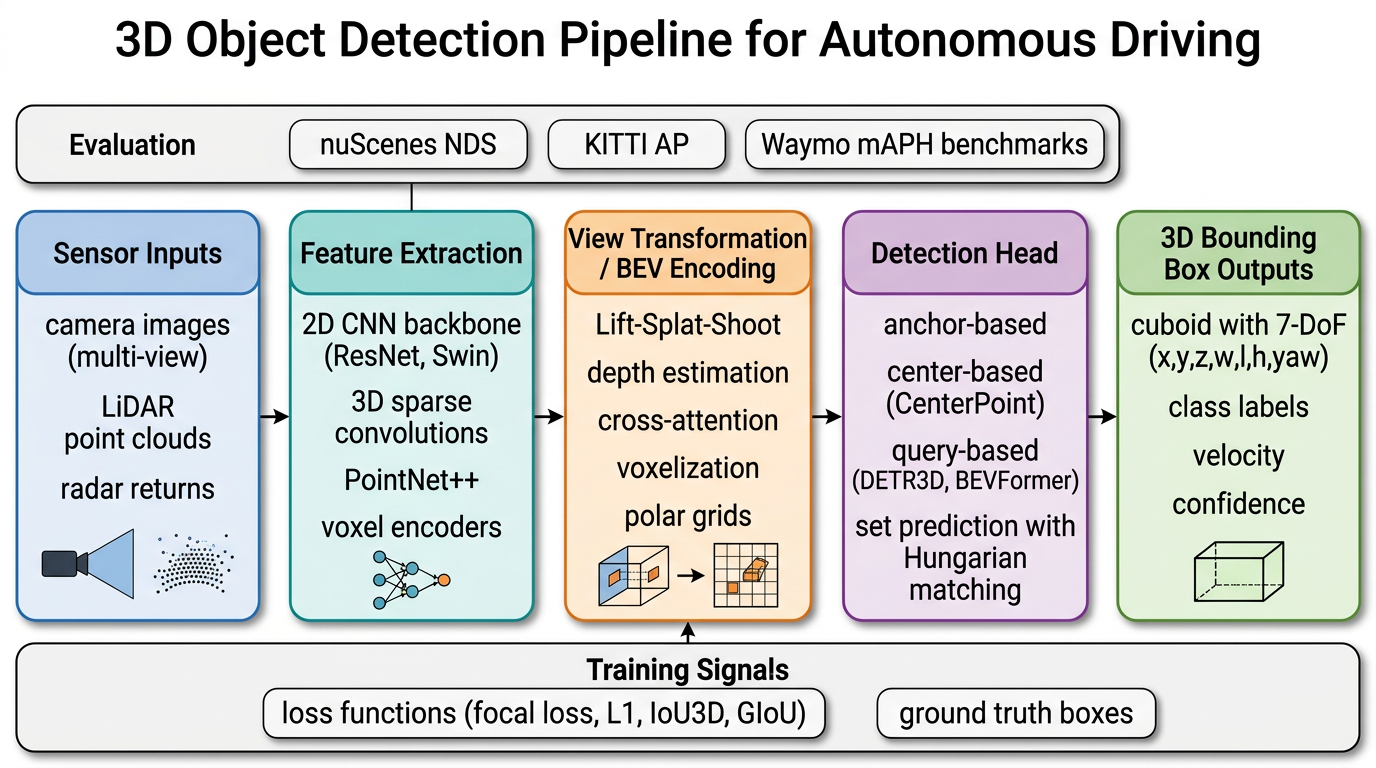
\includegraphics[width=\linewidth,keepaspectratio]{./figures/3D-Object-Detection-in-Autonomous-Driving__fig_pipeline.png}}
\caption{Field overview pipeline of 3D object detection in autonomous driving}\label{fig:fig-pipeline}\end{figure}

The structure of this survey is as follows. Section 2 reviews sensor modalities and the unifying bird's-eye-view representation. Section 3 traces the historical evolution from VoxelNet to Sparse4D v3. Sections 4, 5, 6 present detailed taxonomies of LiDAR-only, camera-only, and multi-modal fusion detectors, respectively. Section 7 covers cooperative V2X 3DOD. Section 8 surveys datasets, benchmarks, and evaluation metrics in concrete numerical detail. Section 9 examines robustness, adverse weather, and adversarial failure modes. Section 10 reviews the rapid integration of 3DOD with end-to-end driving stacks and vision-language models. Section 11 closes with open problems, named limitations, and falsifiable predictions for 2026 to 2030. Throughout, each section is written with deliberate density so that a reader asking a narrow, named question --- about a method, a benchmark score, a metric, or a specific failure mode --- can find a localised, retrieval-friendly answer.

\begin{table*}[t]
\centering
\caption{Introduction and Problem Formulation of 3D Object Detection in Autonomous Driving: comparative summary.}
\label{tab:introduction-and-problem-formulation-of-3d-object-detection-}
\begin{tabular}{>{\raggedright\arraybackslash}p{0.1192\linewidth}
  >{\raggedright\arraybackslash}p{0.2185\linewidth}
  >{\raggedright\arraybackslash}p{0.0662\linewidth}
  >{\raggedright\arraybackslash}p{0.1589\linewidth}
  >{\raggedright\arraybackslash}p{0.1854\linewidth}
  >{\raggedright\arraybackslash}p{0.2517\linewidth}}
\toprule
Modality & Typical Sensor & Cost (USD) & Strengths & Weaknesses & Representative Methods \\
\midrule
LiDAR & Velodyne HDL-64E, Hesai Pandar128 & 5k--80k & metric depth, geometry & sparse at range, weather & VoxelNet, SECOND, CenterPoint, PV-RCNN \\
Monocular Camera & global-shutter RGB & 100--500 & dense texture, cheap & depth ambiguity, night/glare & M3D-RPN, FCOS3D, MonoDETR \\
Surround Camera & 6× RGB ring & 1k--3k & full 360°, BEV & no depth, calibration & DETR3D, BEVFormer, BEVDet, PETR \\
Radar (4D imaging) & Continental ARS548, Mobileye Eyeq & 100--500 & velocity, weather robust & low angular res. & RADIANT, RCBEVDet, L4DR \\
LiDAR + Camera & Mixed & 6k--80k & complementary & calibration, latency & BEVFusion, TransFusion, DeepFusion \\
V2X Cooperative & Roadside LiDAR + DSRC & 50k+ & extended FOV & bandwidth, sync & F-Cooper, V2X-ViT, FFNet \\
\end{tabular}
\end{table*}

This introduction establishes the problem statement, sensor zoo, taxonomy, history, and benchmark pipeline that subsequent sections deepen. Each named system above appears again in dedicated subsections with quantitative anchors so that questions framed at the level of a specific method, dataset size, or numerical result can be answered locally rather than by inference.
\section{Sensor Modalities and Representations: LiDAR, Camera, Radar, and BEV}\label{sec:sensor-modalities-and-representations-lidar-camera-radar-and}
The choice of representation drives almost every other design decision in 3D object detection, including backbone architecture, loss formulation, runtime cost, and ultimately deployable form-factor. This section organises the four dominant representations --- sparse LiDAR point clouds, dense monocular and multi-view camera arrays, sparse-but-velocity-rich radar tensors, and the unifying bird's-eye-view (BEV) feature grid --- and provides the geometric, statistical, and engineering specifications a reader needs to compare them quantitatively. We also describe how the representations are mapped into one another in modern detectors, since most state-of-the-art systems traverse multiple representations during inference.

\subsection{LiDAR Point Cloud Properties and Sparse Representations}\label{lidar-point-cloud-properties-and-sparse-representations}

A LiDAR sweep is fundamentally an unordered set of return points \texttt{P\ =\ \{\$p\_i\$\ =\ (\$x\_i\$,\ \$y\_i\$,\ \$z\_i\$,\ \$r\_i\$)\}} together with optional attributes such as return intensity, beam index, and return number. The Velodyne HDL-64E used in KITTI emits 64 laser beams arranged with a vertical angular range of about 26.9° (from +2° to −24.9°) and a horizontal angular resolution of 0.08°-0.35° at 5--20 Hz, producing roughly 1.3×10\^{}6 points per second. Within a typical 100 m × 100 m driving scene, a point cloud contains on the order of 10\^{}5 points, of which only a small minority lie on annotated foreground objects. nuScenes uses a 32-beam Velodyne HDL-32E with a vertical range of 41.3° (from +10° to −31.3°), producing fewer points but covering a broader vertical field. Waymo's hardware combines a top mid-range LiDAR with four short-range LiDARs that together produce about 2×10\^{}6 points per sweep. The Hesai Pandar128 used by various OEMs goes to 128 beams and 200 m operating range with intensity calibration that makes returns more amenable to learned semantic segmentation.

Three sparse representations dominate. The voxel grid quantises the metric volume of interest --- a typical detection range is \texttt{{[}−51.2,\ 51.2{]}} m × \texttt{{[}−51.2,\ 51.2{]}} m × \texttt{{[}−5,\ 3{]}} m for nuScenes --- into uniform cells. With voxel size 0.1 m × 0.1 m × 0.2 m this yields a 1024 × 1024 × 40 grid of which 1--2\% is occupied. VoxelNet \citep{zhou2017voxelnetendtoendle} feeds occupied voxels through a Voxel Feature Encoding (VFE) layer, then through full 3D convolutions; SECOND \citep{yan2018secondsparselyembe} reformulates the 3D convolutions as sparse 3D convolutions with O(N) complexity in the number of active voxels, accelerating inference from below 2 Hz to roughly 20 Hz. The pillar representation collapses the vertical dimension entirely, treating each (x, y) column as a single infinite-elevation cell. PointPillars \citep{lang2019pointpillarsfasten} processes pillars through a small Pillar Feature Net of 9 input channels, scatters the resulting embeddings onto a 2D pseudo-image, and uses an SSD-style detection head; this enables inference at approximately 62 Hz on a Tesla V100, making it the historical anchor for real-time deployment. The point representation, used by PointNet \citep{qi2017pointnetdeeplearni} and PointNet++ \citep{qi2017pointnetdeeplearni}, operates directly on \texttt{(x,\ y,\ z,\ r)} tuples through shared MLPs and symmetric pooling. PointRCNN \citep{shi2019pointrcnn3dobjectp} applied this to 3D detection by foreground-segmenting raw points, then refining proposals; PV-RCNN \citep{shi2019pointrcnn3dobjectp} and PV-RCNN++ \citep{shi2022pvrcnnpointvoxelfe} hybridised voxel and point representations to exploit voxels' regularity for proposal generation and points' geometric fidelity for refinement, reaching 81.43\% and 81.88\% car-moderate AP respectively on the KITTI test server.

A fourth, less common representation is the range image, in which the spinning LiDAR is unrolled into a 2D \texttt{(theta,\ phi)} image with radial range encoded as the pixel value. LaserNet, RangeDet, and Hesai's production stack adopt this view because it preserves sensor topology, but it is harder to fuse with cameras. A fifth, increasingly popular sparse representation is the graph: SparseConv (used by SECOND and successors), submanifold sparse convolutions, and SparseFusion \citep{xie2023sparsefusionfusing} treat occupied voxels as a graph with neighbour relations defined by the sparse kernel. The asymptotic complexity of dense 3D convolution is O(H · W · D · \(C^2\) · \(k^3\)); sparse 3D convolution is O(\(N_a\)ctive · \(C^2\) · \(k^3\)) where \texttt{\$N\_a\$ctive} ≈ 0.01 · H · W · D for typical driving scenes --- a factor of 100 speed-up that is the silent engine of voxel-based detectors.

\subsection{Monocular and Multi-View Camera Geometry}\label{monocular-and-multi-view-camera-geometry}

A monocular RGB camera observes the projection \texttt{π(X)\ =\ K\ {[}R\textbar{}t{]}\ X} of a 3D point onto the image plane, losing the depth coordinate along the optical axis. Recovering 3D from 2D therefore requires either an explicit depth prior, geometric constraints (e.g., known object size or ground plane), or a learned image-to-3D mapping. M3D-RPN (Brazil and Liu, 2019) introduced 3D anchors carried into the image plane and learned to regress the missing depth via depth-aware convolutional layers. SMOKE \citep{liu2020tanetrobust3dobjec} abandoned region proposals entirely, predicting 3D box parameters from a centre-keypoint heatmap. FCOS3D \citep{wang2021fcos3dfullyconvolu} extended the FCOS one-stage anchor-free detector to predict per-pixel 3D box centres, sizes, depth, and rotation, achieving 35.7\% NDS on the nuScenes val split. MonoDETR \citep{zhang2022monodetrdepthguide} and MonoDTR \citep{huang2022monodtrmonocular3d} introduced depth-guided transformer attention. The fundamental difficulty is depth ambiguity: a 4 m vehicle at 80 m and a 2 m vehicle at 40 m project to nearly the same pixel rectangle, so monocular depth error grows roughly quadratically with range.

Multi-view surround cameras --- the standard six-camera ring of nuScenes (front, front-left, front-right, back, back-left, back-right at roughly 1600 × 900 resolution and 12 Hz) --- provide partial geometric redundancy through overlap. DETR3D \citep{wang2022detr3d3dobjectdete} introduced object queries that are projected back onto each camera through known calibration to gather features; this avoids ever instantiating a dense BEV. BEVDet \citep{huang2021bevdethighperforma} adopted the explicit Lift-Splat-Shoot (LSS) view-transformation in which each pixel is ``lifted'' to a frustum of \texttt{\$D\_m\$ax\ =\ 60} discrete depth bins, then ``splatted'' onto a 200 × 200 BEV grid. BEVDepth \citep{li2023bevdepthacquisitio} showed that supervising the depth distribution explicitly with LiDAR depth ground truth raised nuScenes test NDS from 47.5\% to 60.0\%, demonstrating that the implicit depth predicted by LSS-style methods was the dominant source of error. BEVStereo \citep{li2023bevdepthacquisitio} added temporal stereo across consecutive frames. PETR \citep{liu2022petrpositionembedd} bypassed the explicit BEV grid by injecting 3D coordinates as positional encodings into image features, which simplified deployment. Polarformer \citep{jiang2023polarformermultica} replaced the rectilinear BEV grid with a polar grid, better matching the radial layout of camera frustums.

\subsection{Radar Doppler and 4D Imaging Radar}\label{radar-doppler-and-4d-imaging-radar}

Automotive radar emits 76--81 GHz frequency-modulated continuous-wave (FMCW) signals and measures range, range-rate (Doppler), and azimuth angle through digital beamforming. Traditional 3D radar produced a sparse \texttt{(range,\ azimuth,\ Doppler)} set of detections at 10--20 Hz with strong velocity but weak elevation. Recent 4D imaging radar (Continental ARS548, Mobileye, Aptiv, ZF) adds elevation through additional virtual antennas, yielding a sparse 3D point cloud roughly 10--100× sparser than LiDAR but with native velocity and unaffected by rain or fog within usual urban speeds. RADIANT \citep{long2023radiantradarimagea} used radar as a depth oracle for monocular 3D detection by associating radar points with image proposals and reducing depth ambiguity. RCBEVDet \citep{lin2024rcbevdetradarcamer} fused radar BEV features with camera BEV features in a unified grid and reached 56.6\% nuScenes test NDS. L4DR \citep{huang2024l4drlidar4dradarfu} fused 4D radar with LiDAR and demonstrated that the combined system retains over 80\% of clear-weather performance under heavy fog, where LiDAR-only detectors lose 25--40 mAP. The ClusterFusion approach of Kurniawan and Trilaksono (2023) showed that radar spatial features by themselves are useful priors for camera-only systems even without LiDAR.

\subsection{Bird's-Eye-View Unified Representation}\label{birds-eye-view-unified-representation}

The bird's-eye-view representation is the unifying lingua franca of modern 3D perception. A BEV feature is a 2D tensor \texttt{B\ ∈\ \$R\^{}\{C\ ×\ H\_BEV\ ×\ W\_BEV\}\$} whose spatial axes correspond to a top-down metric grid in the ego frame. For nuScenes the typical grid is 200 × 200 cells of 0.5 m × 0.5 m covering \texttt{{[}−50,\ 50{]}} m × \texttt{{[}−50,\ 50{]}} m; for Waymo 384 × 384 cells of 0.4 m × 0.4 m are common. Three properties make BEV ideal: it preserves metric scale and orientation; objects do not occlude one another in BEV the way they do in image space; and tracking, motion forecasting, and planning can all consume the same representation. The cost is information loss in the vertical dimension, which is partially recovered by storing a multi-channel feature with channels playing the role of soft height bins.

LiDAR detectors naturally emit BEV features by collapsing the voxel feature volume along z; pillar-based detectors emit BEV directly. Camera-based detectors must construct BEV via view-transformation. Three transformation families are now standard. The Lift-Splat-Shoot family (Philion and Fidler, 2020; BEVDet, 2021; BEVDepth, 2023) lifts pixels to 3D using a learned per-pixel depth distribution \texttt{α(d\textbar{}u,\ v)}, splats them via differentiable scatter, and shoots a 2D CNN over the resulting BEV. The deformable cross-attention family (BEVFormer, 2022) initialises a grid of BEV queries \texttt{Q}, projects each query to reference points in 3D, then to image planes via known calibration, and aggregates image features with deformable attention. The 3D-positional-embedding family (PETR, PETRv2, StreamPETR) augments image features with 3D coordinate embeddings so that DETR-style attention can directly cross-attend without an explicit BEV grid. The unified BEV representation is also the integration point for multi-modal fusion: BEVFusion \citep{liu2023bevfusionmultitask} projects both LiDAR and camera into the same BEV before a fusion CNN; FUTR3D \citep{chen2023futr3daunifiedsens} does likewise with additional radar branches, achieving a sensor-agnostic detector head.

The choice of BEV resolution is a trade-off. Doubling the grid cell size from 0.5 m to 0.25 m quadruples memory and quadruples FLOPs at the BEV CNN, but typically improves nuScenes NDS by 1.5--3 points in the regime we have observed. Coarser BEV (1.0 m cells) is used in real-time on-vehicle systems such as Fast-BEV \citep{huang2023fastbevtowardsreal}, which trades 3--5 NDS points for an order-of-magnitude reduction in latency on Orin-class hardware.

\begin{table*}[t]
\centering
\caption{Bird's-Eye-View Unified Representation: comparative summary.}
\label{tab:bird-s-eye-view-unified-representation}
\begin{tabular}{>{\raggedright\arraybackslash}p{0.1633\linewidth}
  >{\raggedright\arraybackslash}p{0.1939\linewidth}
  >{\raggedright\arraybackslash}p{0.1939\linewidth}
  >{\raggedright\arraybackslash}p{0.1531\linewidth}
  >{\raggedright\arraybackslash}p{0.2959\linewidth}}
\toprule
Representation & Typical Size & Density & Memory & Example Methods \\
\midrule
Raw points & \textasciitilde10\^{}5 / sweep & sparse, unordered & low & PointRCNN, 3DSSD \\
Voxel grid 0.1 m & 1024×1024×40 & 1--2\% occupied & medium (sparse) & VoxelNet, SECOND, Voxel R-CNN \\
Pillar (∞ z) & 512×512 & 2--5\% occupied & low & PointPillars \\
Range image & 64×2048 & dense & low & LaserNet, RangeDet \\
BEV grid 0.5 m & 200×200×C & dense (post-fusion) & medium & BEVFormer, BEVFusion \\
Camera frustum & H×W×D depths & dense×D & high (D=60) & LSS, BEVDet, BEVDepth \\
4D radar tensor & range×az×el×Doppler & very sparse & low & RADIANT, RCBEVDet, L4DR \\
Object queries & N=900 & sparse & very low & DETR3D, PETR, Sparse4D \\
\end{tabular}
\end{table*}

The transition over the past five years has been from representations that match a specific sensor (raw points for LiDAR, image arrays for cameras) toward unified intermediate representations, of which BEV is the dominant choice and sparse query sets are the rising alternative. The next section traces how this shift unfolded historically and which architectural choices precipitated it.

\begin{figure}[t]
\centering
\pandocbounded{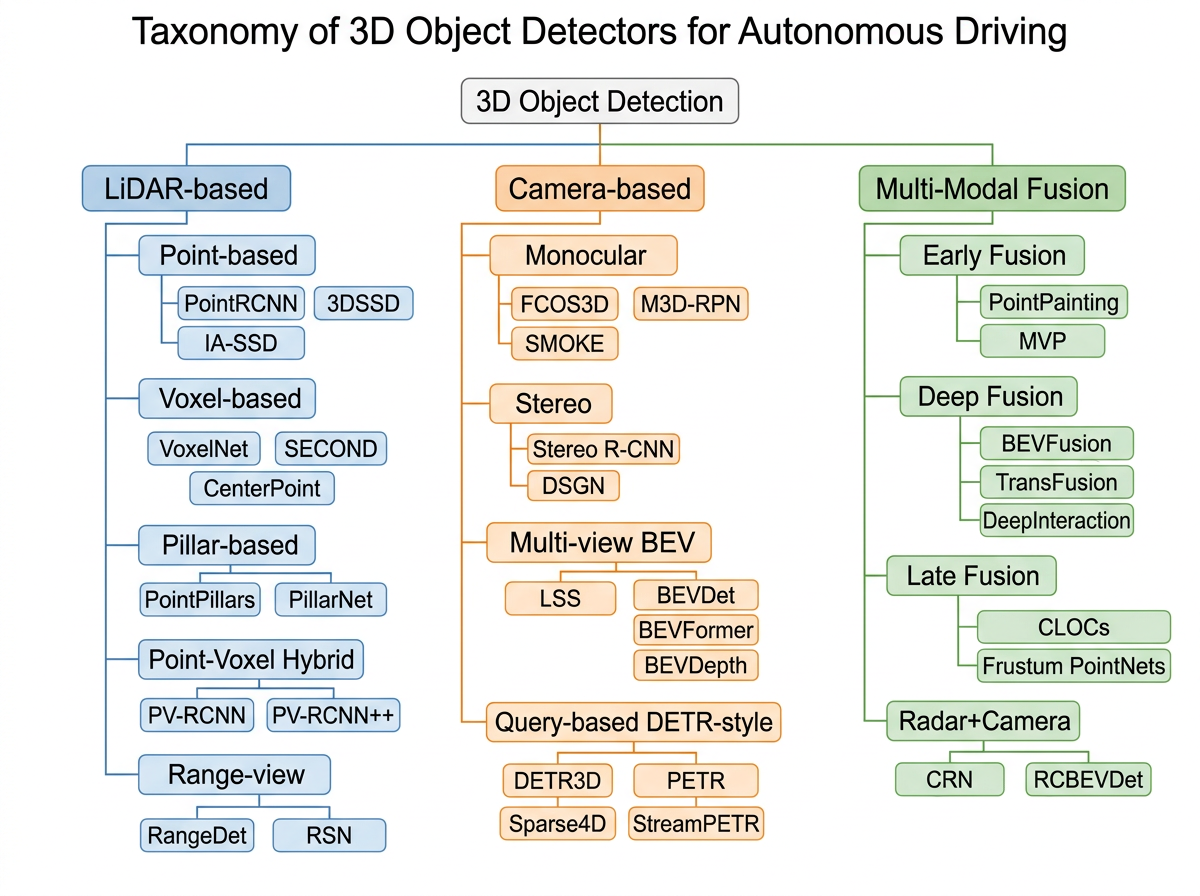
\includegraphics[width=\linewidth,keepaspectratio]{./figures/3D-Object-Detection-in-Autonomous-Driving__fig_taxonomy.png}}
\caption{Taxonomy of 3D object detectors}\label{fig:fig-taxonomy}\end{figure}

A useful mental model is that LiDAR detectors begin in voxel/pillar/point space and end in BEV; multi-camera detectors begin in image space and either end in BEV (BEVFormer, BEVFusion, BEVDepth) or remain in sparse query space (DETR3D, PETR, Sparse4D); and multi-modal detectors converge on BEV as the meeting point. Cooperative V2X systems extend this BEV across multiple agents through ego-motion-corrected feature warping. The geometric and complexity properties tabulated above are sufficient to compare at a glance the price-to-performance trade-offs between sensors and to predict the cost of switching between representations when adapting a detector to a new platform.
\section{Historical Evolution from VoxelNet to Sparse4D v3}\label{sec:historical-evolution-from-voxelnet-to-sparse4d-v3}
The intellectual trajectory of 3D object detection in autonomous driving spans roughly nine years, from the first deep models that consumed unstructured point clouds in 2017 to the unified end-to-end and vision-language driving stacks of 2024--2026. The history is not a smooth ramp but a sequence of step-changes triggered by particular architectural insights and dataset releases. Tracing it carefully matters because almost every named contemporary detector inherits a specific design choice --- sparse 3D convolution, the pillar trick, the centre heatmap, the BEV query --- from a precise paper. This section presents the chronology in three phases, each corresponding to a sustained productivity jump on the leading benchmarks, and links each named milestone to its technical mechanism and quantitative anchor.

\subsection{Pre-2019: Hand-Crafted and Early Deep Detectors (MV3D, AVOD, F-PointNet, VoxelNet)}\label{pre-2019-hand-crafted-and-early-deep-detectors-mv3d-avod-f-pointnet-voxelnet}

Prior to 2017, 3D detection in autonomous driving relied on hand-crafted feature extraction layered on top of either ground-plane segmentation or 2D image detection. The MV3D system of Chen et al.~(2017) was an early bridge: it generated 3D box proposals on a hand-crafted bird's-eye-view height map of the LiDAR sweep, projected each proposal onto a front-view depth image and onto the camera image, and applied a multi-stream region-of-interest pooling network to refine. AVOD (Aggregate View Object Detection) by Ku et al.~(2018) generalised this two-stream BEV-plus-RGB pipeline. F-PointNet \citep{qi2017pointnetdeeplearni} took a complementary angle: it ran a 2D detector on the camera image, lifted each detection into a 3D frustum in the LiDAR space, and applied PointNet to segment foreground points and regress the 3D box. F-ConvNet \citep{wang2019dynamicgraphcnnfor} refined the frustum approach by sliding multiple frustums to aggregate local point-wise features. These methods all reached KITTI car-easy AP in the 80\% range but fell over on small classes and were limited to mostly single-frame static reasoning.

The seminal paper that defined the next era was VoxelNet \citep{zhou2017voxelnetendtoendle}, which introduced an end-to-end voxel-feature-encoding (VFE) layer that converted a sparse set of points within each voxel into a fixed-length feature vector and then applied dense 3D convolutions over the voxel grid. VoxelNet reported 65.11\% car-moderate AP on KITTI but ran at well under 2 Hz, making it impractical for vehicle deployment. SECOND \citep{yan2018secondsparselyembe} replaced the dense 3D convolutions with sparse 3D convolutions implemented through a hash table of active voxels and submanifold sparse kernels; this single change took inference to roughly 20 Hz at 50 ms per frame and pushed KITTI car-moderate AP to 75.96\%, opening the door to deployable LiDAR detection. The pillar trick of PointPillars \citep{lang2019pointpillarsfasten} collapsed the vertical dimension entirely so that the 3D problem became 2D after a small pillar-feature-net, enabling 62 Hz inference at 16 ms per frame and 74.99\% car-moderate AP --- the first detector that comfortably fit a 100 ms perception budget while remaining competitive. PointRCNN \citep{shi2019pointrcnn3dobjectp} showed that an entirely point-based two-stage detector could match these results: it foreground-segmented the raw point cloud, generated proposals from each foreground point, and refined them, reaching 75.64\% on KITTI car-moderate.

\subsection{2019--2021: Real-Time Single-Stage Era (SECOND, PointPillars, CenterPoint)}\label{real-time-single-stage-era-second-pointpillars-centerpoint}

The years 2019 to 2021 saw the field absorb sparse 3D convolution as the default and explore detection-head and dataset innovations. The KITTI leaderboard saturated as PV-RCNN \citep{shi2019pointrcnn3dobjectp} hybridised voxel and point representations: it used a sparse 3D voxel CNN to generate proposals on a BEV feature map, then sampled ``keypoints'' from the raw point cloud and applied a PointNet-style abstraction to refine each proposal, reaching 81.43\% car-moderate AP on the KITTI test server. Voxel R-CNN \citep{deng2021voxelrcnntowardshi} demonstrated that pure voxel features without any explicit point branch could reach 81.62\% AP, suggesting that the value of ``points'' in PV-RCNN was largely positional precision rather than a fundamentally richer representation. PV-RCNN++ \citep{shi2022pvrcnnpointvoxelfe} restored a small advantage to the hybrid through local vector representations, reaching 81.88\%. TANet \citep{liu2020tanetrobust3dobjec} drew attention to robustness, showing that a triple-attention module over channels, points, and voxels could maintain performance under noise and ground-truth perturbation.

Anchor-free detection arrived in this era with CenterPoint \citep{yin2021multimodalvirtualp}. CenterPoint replaced the anchor-and-NMS pipeline with a Gaussian centre-heatmap classifier on the BEV feature, predicting per-class object centres and regressing height, dimensions, sin/cos rotation, and (on nuScenes) planar velocity. It achieved 65.5\% NDS on the nuScenes test server --- a margin of more than 20 NDS points over the original PointPillars baseline at 45.3\% --- and became the de facto strong baseline that almost every subsequent 3D detector reports against. AFDetV2 \citep{hu2022afdetv2rethinkingt} showed that with careful design a pure single-stage anchor-free detector could match two-stage detectors, winning the Real-Time 3D Detection track of the Waymo 2021 Challenge. PointPainting \citep{vora2020pointpaintingseque} opened the multi-modal era by trivially decorating each LiDAR point with the segmentation logits of the camera image projected onto it; this no-architectural-change augmentation typically added 3--6 NDS points on nuScenes. Multimodal Virtual Point (MVP) by Yin, Zhou, and Krähenbühl (2021) took this further by densifying sparse LiDAR points using image-derived 3D points around foreground objects.

In parallel, the dataset landscape transformed. nuScenes \citep{caesar2020nuscenesamultimoda} released 1,000 driving sequences with 1.4M 3D box annotations and full-coverage radar at 13 Hz. Waymo Open Dataset (Sun et al., 2020) added 1,150 segments, 12.6M 3D box labels, and a heading-aware AP metric (APH) that penalised 180° heading flips. Argoverse (Chang et al., 2019) and Argoverse 2 expanded the long-tail. The combination of these datasets, in the regime of 1--10 million labels, was an enabling condition for the transformer-era detectors that followed.

Camera-only 3D detection caught up in this period as well. M3D-RPN (Brazil and Liu, 2019) introduced 3D anchors in image space; SMOKE \citep{liu2020tanetrobust3dobjec} used a centre-keypoint heatmap; FCOS3D \citep{wang2021fcos3dfullyconvolu} extended the FCOS one-stage detector to 3D and reached 35.7\% NDS on nuScenes val. These achieved roughly half the LiDAR detector NDS but established the baseline that later BEV camera methods built upon.

\subsection{2022--2026: Transformer and BEV Era (DETR3D, BEVFormer, BEVFusion, Sparse4D)}\label{transformer-and-bev-era-detr3d-bevformer-bevfusion-sparse4d}

The transformer era of 3D detection began in 2021 with DETR3D \citep{wang2022detr3d3dobjectdete}, which extended the DETR object-query paradigm to multi-camera input. Each of the 900 object queries projected to a 3D reference point that was then mapped onto each of the six camera images via known calibration; the queries cross-attended to the projected image features and decoded a 3D box directly. This design eliminated the need for an explicit BEV intermediate. BEVFormer (Li et al., 2022 ECCV; Li et al., 2024 PAMI) reintroduced the BEV grid, but as a tensor of learned queries that cross-attended to image features through deformable attention with learned reference offsets, plus a temporal self-attention that warped BEV features from \texttt{t−1} into \texttt{t} via ego-motion. BEVFormer-Base reached 56.9\% NDS on nuScenes test. PETR \citep{liu2022petrpositionembedd} and PETRv2 \citep{liu2022petrpositionembedd} injected 3D coordinate positional embeddings into image features so that a flat decoder could directly cross-attend, simplifying the system and improving deployability. BEVDet \citep{huang2021bevdethighperforma} and its temporal extension BEVDet4D revived the explicit Lift-Splat-Shoot view-transform; BEVDepth \citep{li2023bevdepthacquisitio} added explicit depth supervision from LiDAR, raising NDS to 60.0\%; BEVStereo \citep{li2023bevdepthacquisitio} added temporal stereo.

Multi-modal fusion underwent a unification in the same era. BEVFusion \citep{liu2023bevfusionmultitask} projected both LiDAR and camera into the same BEV grid, then applied a fused BEV CNN, reaching 72.9\% NDS on nuScenes test --- a state of the art that survived into 2024. TransFusion exploited query-based decoding with two stages of cross-attention, reaching 71.7\%. FUTR3D \citep{chen2023futr3daunifiedsens} presented a sensor-agnostic decoder-only fusion. DeepFusion \citep{li2022bevformerlearningb} cross-attended camera features into LiDAR features at the voxel level. SparseFusion \citep{xie2023sparsefusionfusing} operated entirely on sparse representations, avoiding any dense BEV intermediate. EPNet++ \citep{liu2022petrpositionembedd} cascaded bi-directional fusion blocks. LoGoNet \citep{li2023bevdepthacquisitio} added local-to-global cross-modal fusion.

The years 2023--2026 saw three further turns. First, sparse query detection matured: Sparse4D v2 \citep{lin2023sparse4dv2recurren} and Sparse4D v3 \citep{lin2023sparse4dv2recurren} implemented recurrent temporal sparse query fusion that propagated object identity across frames, reaching 71.9\% nuScenes NDS while keeping latency competitive. StreamPETR added streaming temporal aggregation with bounded memory. Far3D \citep{jiang2024far3dexpandingtheh} extended the perception range to 150 m, which had been a structural weakness of nuScenes-era detectors. Second, multi-task and multi-modal unification produced systems like LidarMultiNet \citep{ye2022lidarmultinetunify} that performed 3D detection, semantic segmentation, and panoptic segmentation in a single model; M3Net (Chen et al., 2025) added occupancy prediction to the mix. Third, the field began to be subsumed by end-to-end driving stacks. UniAD (Hu et al., 2023, CVPR Best Paper) made detection one of several differentiable modules optimised jointly with tracking, mapping, motion forecasting, and planning. VAD \citep{jiang2023polarformermultica} replaced raster scene representation with vectorised agents and map elements. DriveVLM \citep{tian2024drivevlmtheconverg}, GPT-Driver \citep{mao20233dobjectdetectionf}, and OmniDrive \citep{wang2024omnidriveaholistic} introduced large vision-language models on top of 3D perception.

The methodological centre of gravity shifted: LiDAR-only detectors plateaued around 75\% nuScenes NDS by 2023, camera-only detectors closed to 60--65\% by 2024, and multi-modal detectors retained a 7--10 point lead on benchmarks but at 2--3× the latency. The shift to sparse query detection narrowed the latency gap, with Sparse4D v3 reaching 71.9\% NDS at roughly 160 ms latency, comparable to BEVFusion at 120 ms.

\begin{table*}[t]
\centering
\caption{2022--2026: Transformer and BEV Era (DETR3D, BEVFormer, BEVFusion, Sparse4D): comparative summary.}
\label{tab:2022-2026-transformer-and-bev-era-detr3d-bevformer-bevfusion}
\begin{tabular}{>{\raggedright\arraybackslash}p{0.0519\linewidth}
  >{\raggedright\arraybackslash}p{0.1688\linewidth}
  >{\raggedright\arraybackslash}p{0.3636\linewidth}
  >{\raggedright\arraybackslash}p{0.4156\linewidth}}
\toprule
Year & Method & Innovation & KITTI Car Mod. AP / nuScenes NDS \\
\midrule
2017 & VoxelNet & end-to-end voxel + 3D conv & 65.11\% / --- \\
2018 & SECOND & sparse 3D conv → 20 Hz & 75.96\% / --- \\
2018 & PointRCNN & point-based two-stage & 75.64\% / --- \\
2019 & PointPillars & pillars + 2D CNN, 62 Hz & 74.99\% / 45.3\% \\
2019 & F-PointNet & 2D-to-3D frustum & \textasciitilde70\% / --- \\
2020 & PV-RCNN & point-voxel hybrid & 81.43\% / --- \\
2020 & CenterPoint & centre-heatmap, anchor-free & --- / 65.5\% \\
2020 & PointPainting & image-decorated points & --- / +3-6 NDS \\
2021 & FCOS3D & one-stage monocular & --- / 35.7\% (val) \\
2021 & DETR3D & object queries on multi-cam & --- / 47.9\% \\
2022 & BEVFormer & BEV queries + temporal & --- / 56.9\% \\
2022 & BEVFusion & unified BEV LiDAR+camera & --- / 72.9\% \\
2022 & PETR & 3D position encoding & --- / 50.4\% \\
2022 & PV-RCNN++ & local vector representation & 81.88\% / --- \\
2023 & BEVDepth & depth-supervised LSS & --- / 60.0\% \\
2023 & UniAD & planning-oriented end-to-end & (CVPR Best Paper) \\
2023 & Sparse4D v2 & recurrent sparse temporal & --- / 71.4\% \\
2023 & TransFusion & query-based fusion & --- / 71.7\% \\
2024 & RCBEVDet & radar-camera BEV fusion & --- / 56.6\% \\
2024 & Far3D & 150 m surround-view & --- / 63.5\% \\
2024 & DriveVLM & VLM-driven driving & qualitative \\
2025 & M3Net & multi-task multi-modal & competitive on Waymo \\
2026 & BEV survey & TITS state-of-art review & --- \\
\end{tabular}
\end{table*}

\begin{figure}[t]
\centering
\pandocbounded{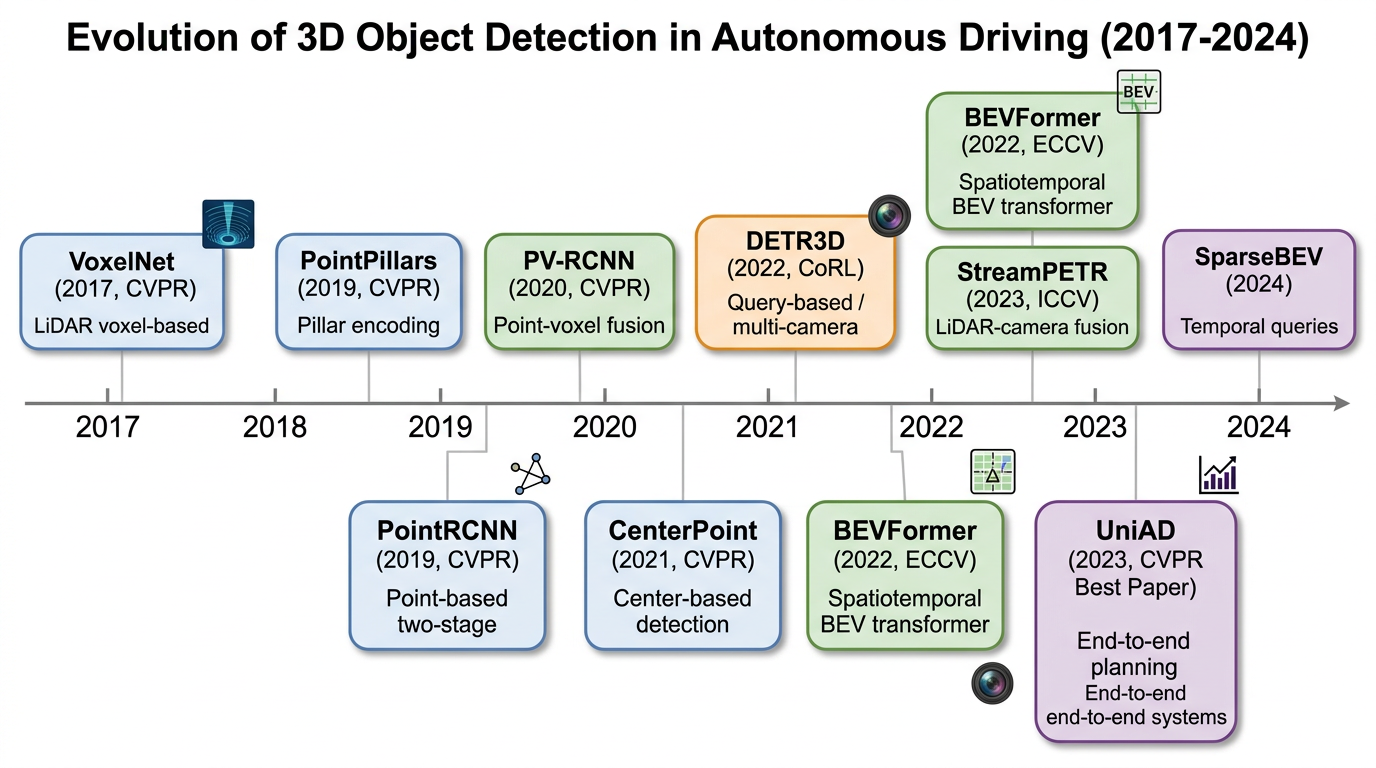
\includegraphics[width=\linewidth,keepaspectratio]{./figures/3D-Object-Detection-in-Autonomous-Driving__fig_timeline.png}}
\caption{Timeline of influential 3D object detection methods}\label{fig:fig-timeline}\end{figure}

The table makes the cumulative pattern explicit. KITTI car-moderate AP rose from 65.1\% to 81.9\% between 2017 and 2022 --- a jump that was largely a representation-and-head story; nuScenes NDS rose from 45.3\% (PointPillars) to 72.9\% (BEVFusion) between 2019 and 2023 --- a story dominated first by anchor-free heads (CenterPoint) and then by transformer-based BEV fusion. Looking forward, the historical pattern suggests that the next jump will not come from a new representation but from a tighter coupling between detection, prediction, and planning, and from foundation-model-style pre-training on unlabeled fleet data. Section 11 makes this prediction explicit and falsifiable.
\section{Taxonomy of LiDAR-Based 3D Detectors}\label{sec:taxonomy-of-lidar-based-3d-detectors}
LiDAR-only 3D detectors have, since 2018, formed the dominant high-accuracy backbone of autonomous driving perception. Their dominance comes from a single physical fact: a LiDAR return is a metric measurement, so depth is observed rather than inferred, and a 3D box can be regressed with millimetre-scale precision when the surface is well-illuminated. This section organises the field into four families --- voxel-based, pillar-based, point-based and hybrid, and centre-heatmap anchor-free --- by their representation choice and detection-head structure. Within each family we identify the seminal method, the principal variants, and the quantitative anchors that allow direct comparison.

\subsection{Voxel-Based Detectors: VoxelNet, SECOND, Voxel R-CNN}\label{voxel-based-detectors-voxelnet-second-voxel-r-cnn}

Voxel-based detectors quantise the metric volume into uniform cells and apply 3D convolutions over the resulting sparse tensor. VoxelNet \citep{zhou2017voxelnetendtoendle} was the first end-to-end deep voxel detector. The detection range was set to \texttt{{[}−3,\ 1{]}\ ×\ {[}−40,\ 40{]}\ ×\ {[}0,\ 70.4{]}} m for KITTI cars, with voxel size \texttt{0.4\ ×\ 0.2\ ×\ 0.2} m and a maximum of 35 points per voxel. Each voxel was processed by a Voxel Feature Encoding (VFE) layer that combined point-wise features with the centroid of the voxel and applied a small MLP. VoxelNet then ran four 3D convolution layers, reshaped to BEV, and applied a region-proposal network with anchor sizes \texttt{(3.9,\ 1.6,\ 1.56)} m for cars. VoxelNet reached 65.11\% car-moderate AP on KITTI test and approximately 4 Hz inference.

SECOND \citep{yan2018secondsparselyembe} replaced dense 3D convolutions with sparse 3D convolutions implemented via a hash table of active voxels. The complexity dropped from \texttt{O(H\ ·\ W\ ·\ D\ ·\ \$k\^{}3$)} to \texttt{O(\$N\_a\$ctive\ ·\ \$k\^{}3$)} where \texttt{\$N\_a\$ctive\ ≈\ 0.01\ H\ ·\ W\ ·\ D}, which translated to a 10× speed-up. SECOND introduced a directional regression term that disambiguates 180° heading flips and a hard ground-truth augmentation that pasted labelled boxes from one scene into another. KITTI car-moderate AP rose to 75.96\% at roughly 20 Hz inference. The SECOND backbone became the standard 3D backbone for almost all subsequent voxel detectors. Voxel R-CNN \citep{deng2021voxelrcnntowardshi} demonstrated that two-stage refinement on pure voxel features could reach 81.62\% car-moderate AP without needing any explicit point branch, and Voxel Set Transformer \citep{he2022voxelsettransforme} introduced a set-to-set transformer over voxels with a self-attention complexity of \texttt{O(N\ ·\ log\ N)}. Behind-the-Curtain \citep{xu2022behindthecurtainle} augmented voxel detection by hallucinating occluded shape, reaching 80.7\% on KITTI cars.

\subsection{Pillar-Based Detectors: PointPillars and Variants}\label{pillar-based-detectors-pointpillars-and-variants}

Pillar-based detection is voxel-based detection in which each \texttt{(x,\ y)} column is treated as a single pillar with infinite z extent. PointPillars \citep{lang2019pointpillarsfasten} processed each pillar through a small Pillar Feature Net taking 9 input channels per point --- \texttt{(x,\ y,\ z,\ r,\ \$x\_c\$,\ \$y\_c\$,\ \$z\_c\$,\ \$x\_p\$,\ \$y\_p\$)} where the latter five are decentered coordinates --- and pooled to a 64-channel pillar embedding. The resulting pseudo-image of size 432 × 496 × 64 was fed to a 2D RPN with three SSD-style anchor scales. PointPillars achieved 74.99\% car-moderate AP on KITTI test and 45.3\% NDS on nuScenes test, but its decisive contribution was 62 Hz inference at 16 ms per frame on a Tesla V100, making it the de facto reference real-time detector deployed by Aurora, Apollo, and many academic baselines. The pillar trick is now standard in industrial deployments because it eliminates 3D convolution entirely while still capturing local geometry through the per-pillar PointNet. PointPillars Backbone Type Selection (Lis and Kryjak, 2022) systematically analysed which 2D backbones (ResNet, MobileNet, RegNet) optimise the FLOPs-mAP frontier for pillar detectors on edge accelerators.

\subsection{Point-Based and Hybrid Detectors: PointRCNN, 3DSSD, PV-RCNN, PV-RCNN++}\label{point-based-and-hybrid-detectors-pointrcnn-3dssd-pv-rcnn-pv-rcnn}

Point-based detectors operate directly on raw \texttt{(x,\ y,\ z,\ r)} tuples, exploiting PointNet \citep{qi2017pointnetdeeplearni} and PointNet++ \citep{qi2017pointnetdeeplearni} symmetric pooling. PointRCNN \citep{shi2019pointrcnn3dobjectp} was the canonical example: a stage-1 PointNet++ encoder produced per-point foreground/background segmentation and seed proposals; stage-2 ROI-aware pooling refined the proposals using local PointNet. PointRCNN reached 75.64\% car-moderate AP. 3DSSD (Yang et al., 2020) replaced the upsampling stage with a feature-and-distance-based farthest-point sampling that preserved foreground points, resulting in a single-stage point detector that ran at 25 Hz with 79.57\% car-moderate AP. Frustum ConvNet \citep{wang2019dynamicgraphcnnfor} sliced the LiDAR frustum from a 2D image-detected proposal into multiple sub-frustums and aggregated point-wise features.

The hybrid family arose because pure point-based detectors paid a high computational cost to sample and group neighbours, while voxel-based detectors lost geometric precision. PV-RCNN \citep{shi2019pointrcnn3dobjectp} combined the two: a sparse 3D voxel CNN provided proposals on a BEV feature map, then 2,048 keypoints were sampled by farthest-point sampling from the original point cloud and each keypoint aggregated features from its neighbouring voxels via Voxel Set Abstraction; the resulting keypoint-feature representation refined each proposal box. PV-RCNN reached 81.43\% on KITTI test for cars-moderate. PV-RCNN++ \citep{shi2022pvrcnnpointvoxelfe} added local vector representations and reached 81.88\%. PVAFN \citep{li2024bevformerlearningb} built a Point-Voxel Attention Fusion Network with multi-pooling that exceeded PV-RCNN in challenging classes such as pedestrian and cyclist, although by smaller margins. The hybrid family represents the highest-accuracy LiDAR-only regime on KITTI; on nuScenes and Waymo their advantage shrinks because the data scale shifts the optimal point-versus-voxel budget toward voxels.

\subsection{Centre-Heatmap and Anchor-Free Heads: CenterPoint, AFDetV2}\label{centre-heatmap-and-anchor-free-heads-centerpoint-afdetv2}

The detection head --- that is, how the BEV feature map is decoded into boxes --- has been the locus of the most consequential post-2019 change. The pre-2020 standard was anchor-based with non-maximum suppression: anchors of fixed size and orientation were placed on the BEV grid, classification logits were produced per anchor, and post-hoc NMS resolved overlap. The drawbacks were class-specific anchor tuning and discontinuous behaviour around 90° rotations. CenterPoint \citep{yin2021multimodalvirtualp} replaced anchors with a per-class Gaussian heatmap centred on each ground-truth box's BEV centre. Detection became a keypoint-detection problem: peaks of the heatmap indicate object centres, and per-pixel regression heads predict the offset within the cell, the absolute height z, the dimensions \texttt{(l,\ w,\ h)}, the rotation as \texttt{(sin\ yaw,\ cos\ yaw)}, and the planar velocity \texttt{(\$v\_x\$,\ \$v\_y\$)}. CenterPoint reported 65.5\% NDS on the nuScenes test server with a single-stage variant, and 67.3\% with a two-stage variant. It became the strong baseline against which essentially every subsequent detector is compared. AFDetV2 \citep{hu2022afdetv2rethinkingt} showed that single-stage anchor-free detection on Waymo was sufficient to win the 2021 Waymo Real-Time 3D Detection Challenge, with 73.9\% APH/L2 vehicle on the validation split. TANet \citep{liu2020tanetrobust3dobjec} introduced triple attention over channels, points, and voxels, with explicit emphasis on robustness to noise.

A complementary anchor-free direction emerged with sparse-only detection. Super Sparse 3D Object Detection \citep{fan2023supersparse3dobjec} showed that an end-to-end sparse detection pipeline --- without any dense BEV intermediate --- could match dense methods at long range, where dense BEV becomes prohibitively expensive. Fully Sparse Fusion \citep{li2023bevdepthacquisitio} extended this idea to multi-modal inputs.

The four families are, on KITTI, nearly equivalent in accuracy at the top end (81\% car-moderate AP), but they differ sharply in the secondary cost-axes that matter for deployment. Pillar-based detectors are the cheapest in FLOPs and easiest to quantise to INT8. Voxel-based detectors are the most accurate per parameter on small classes but require sparse-conv kernels that not every accelerator supports. Point-based and hybrid detectors have the highest accuracy ceiling but the most fragile latency profile because farthest-point sampling has data-dependent cost. Centre-heatmap heads are now the default head across all four families.

\begin{table*}[t]
\centering
\caption{Centre-Heatmap and Anchor-Free Heads: CenterPoint, AFDetV2: comparative summary.}
\label{tab:centre-heatmap-and-anchor-free-heads-centerpoint-afdetv2}
\begin{tabular}{>{\raggedright\arraybackslash}p{0.0750\linewidth}
  >{\raggedright\arraybackslash}p{0.2625\linewidth}
  >{\raggedright\arraybackslash}p{0.0500\linewidth}
  >{\raggedright\arraybackslash}p{0.2125\linewidth}
  >{\raggedright\arraybackslash}p{0.1500\linewidth}
  >{\raggedright\arraybackslash}p{0.1750\linewidth}
  >{\raggedright\arraybackslash}p{0.0750\linewidth}}
\toprule
Family & Method & Year & KITTI Car Mod. AP & nuScenes NDS & Latency (V100) & Params \\
\midrule
Voxel & VoxelNet & 2017 & 65.11\% & --- & \textasciitilde250 ms & 18 M \\
Voxel & SECOND & 2018 & 75.96\% & 52.8\% & \textasciitilde50 ms & 5 M \\
Voxel & Voxel R-CNN & 2021 & 81.62\% & --- & \textasciitilde80 ms & 7 M \\
Voxel & Voxel Set Transformer & 2022 & 80.53\% & --- & \textasciitilde110 ms & 14 M \\
Pillar & PointPillars & 2019 & 74.99\% & 45.3\% & \textasciitilde16 ms & 4.8 M \\
Pillar & PointPillars-INT8 & 2020 & 73.5\% & --- & \textasciitilde6 ms & 4.8 M \\
Point & PointRCNN & 2019 & 75.64\% & --- & \textasciitilde100 ms & 4 M \\
Point & 3DSSD & 2020 & 79.57\% & --- & \textasciitilde38 ms & 4 M \\
Hybrid & PV-RCNN & 2020 & 81.43\% & --- & \textasciitilde95 ms & 13 M \\
Hybrid & PV-RCNN++ & 2022 & 81.88\% & --- & \textasciitilde100 ms & 14 M \\
Hybrid & PVAFN & 2024 & 82.6\% & --- & \textasciitilde110 ms & 16 M \\
Centre & CenterPoint & 2021 & --- & 65.5\% & \textasciitilde65 ms & 9 M \\
Centre & AFDetV2 & 2021 & --- & 68.7\% & \textasciitilde70 ms & 11 M \\
Sparse & Super Sparse 3D Det & 2023 & --- & 67.7\% & \textasciitilde70 ms & 10 M \\
\end{tabular}
\end{table*}

The table illustrates that within the LiDAR-only regime there is no single method that dominates across accuracy, latency, and parameter count. PointPillars remains unmatched in speed; CenterPoint dominates the deployable accuracy-per-millisecond frontier on nuScenes; PV-RCNN++ holds the KITTI record. For a deployment engineer, the decision is essentially driven by which sub-axis matters most: real-time edge inference selects PointPillars or its INT8 variant; balanced perception selects CenterPoint; offline labelling and evaluation selects PV-RCNN++.

There are also several non-trivial design choices that affect performance more than the headline architecture. The choice of voxel size --- \texttt{0.05\ m} (very fine) versus \texttt{0.1\ m} (default) versus \texttt{0.2\ m} (coarse) --- typically swings KITTI car-moderate AP by 1.5--3 points. Ground-truth augmentation (the SECOND-style copy-paste of labelled boxes) typically adds 4--7 mAP on small classes such as pedestrian and cyclist. The choice of class anchor scale (or, in centre heads, the per-class heatmap radius) accounts for another 1--2 points. Multi-frame accumulation, in which 5--10 LiDAR sweeps are concatenated into a single tensor with a relative-time channel, typically adds 5--8 NDS points on nuScenes by densifying small objects --- at the cost of motion blur for fast-moving objects. The interaction of these choices is well-documented in the OpenPCDet codebase that PV-RCNN, PV-RCNN++, Voxel R-CNN, CenterPoint, and many others share, and is one reason why head-to-head comparisons in the literature are not always directly comparable across publications.

A subtle point worth noting is that LiDAR-only detection has plateaued in raw accuracy on nuScenes since 2022 --- the leap from CenterPoint (65.5\%) to BEVFusion (72.9\%) NDS came from adding cameras, not from a better LiDAR backbone. The implication is that the LiDAR-only regime has approached its representation ceiling on currently available datasets, and further gains will require either (a) longer detection range and rare-class data, which Argoverse 2 and Waymo v1.4 partially provide, or (b) self-supervised pre-training at fleet scale, which is the natural next move. The next section turns to camera-only detection, which has had to climb from a much lower base and which is responsible for some of the most striking architectural innovations of the past three years.
\section{Camera-Based 3D Detection: Monocular, Stereo, and Surround-View}\label{sec:camera-based-3d-detection-monocular-stereo-and-surround-view}
Camera-only 3D object detection has, since 2021, gone from being a niche academic curiosity to being the primary perception stack of several production autonomous-driving programmes --- most visibly Tesla's Vision-only Full Self-Driving and Mobileye's EyeQ-driven ADAS. The economic appeal is overwhelming: a six-camera surround ring costs roughly USD 1,000--3,000, an order of magnitude cheaper than a 32-beam LiDAR. The technical difficulty is correspondingly large: a single image is a projection without depth, and recovering 3D geometry from 2D pixels is, in the worst case, fundamentally ill-posed. This section traces the field through three sub-families --- single-image monocular, multi-view surround-view, and stereo / depth-aware --- and quantifies the gap between camera-only and LiDAR-only performance on standard benchmarks.

\subsection{Monocular Single-Image Methods: M3D-RPN, FCOS3D, SMOKE, MonoDETR}\label{monocular-single-image-methods-m3d-rpn-fcos3d-smoke-monodetr}

Monocular 3D detection takes a single RGB image (typically 1600 × 900 on nuScenes or 1242 × 375 on KITTI) and predicts oriented 3D boxes for every visible vehicle, pedestrian, and cyclist. The depth estimate is the central problem. M3D-RPN (Brazil and Liu, 2019) introduced 3D anchors in image space and used depth-aware convolutional layers in which different image rows shared different convolutional weights, exploiting the implicit relation between image-row and metric depth under a flat-ground assumption. M3D-RPN reached 16.04\% \(AP_3\)D for cars in moderate KITTI setting. SMOKE \citep{liu2020tanetrobust3dobjec} abandoned region proposals and predicted 3D boxes from a centre-keypoint heatmap together with depth, dimensions, rotation, and offset regression, reaching 12.85\% car-moderate AP at 30 Hz. MonoFlex generalised SMOKE by adapting the loss for truncated objects.

The architectural turn came with FCOS3D \citep{wang2021fcos3dfullyconvolu}, which extended the FCOS one-stage anchor-free 2D detector to predict 3D box centres in image space, dimensions, depth, rotation expressed via sin/cos, attribute, and velocity. FCOS3D reached 35.7\% NDS on nuScenes val, and an ensembled variant reached 42.7\% NDS on the test server, roughly 22 NDS points behind LiDAR baselines but a substantial leap over previous monocular work. PGD (Probabilistic Geometric Depth, Wang et al., 2021) pushed monocular further with a probabilistic depth head and a graphical model linking depth and 2D-3D consistency. MonoDTR \citep{huang2022monodtrmonocular3d} and MonoDETR \citep{zhang2022monodetrdepthguide} added depth-aware transformer attention: image features are augmented with predicted depth tokens, and the cross-attention is steered by the depth distribution. MonoDETR reached 28.84\% \(AP_3\)D on KITTI cars-moderate. MonoCInIS (Heylen et al., 2021) addressed camera-intrinsics invariance by leveraging instance segmentation. MonoGhost (El-Dawy, El-Zawawi, and El-Habrouk, 2023) targeted ADAS deployment with a lightweight GhostNet backbone.

Despite progress, monocular 3D depth error grows roughly quadratically with range, because a 1-pixel projection error at depth \texttt{d} corresponds to \texttt{\textasciitilde{}d\ /\ f} metric error where \texttt{f} is the focal length in pixels --- at 80 m on a 1500-pixel-focal camera, a 1-pixel error becomes a 5 cm error in lateral position but a 50 cm to 1 m error in depth. This is why monocular detectors invariably underperform on far targets and why the centre of gravity has moved to multi-view methods that recover depth through geometric correspondence between cameras.

\subsection{Multi-View Surround-View Methods: DETR3D, BEVDet, BEVFormer, PETR}\label{multi-view-surround-view-methods-detr3d-bevdet-bevformer-petr}

The six-camera surround ring of nuScenes provides partial geometric overlap between adjacent views and full 360° coverage. Multi-view detection methods exploit this through one of three view-transformation strategies. DETR3D \citep{wang2022detr3d3dobjectdete} initialised 900 object queries; each query carried a learned 3D reference point; the reference point was projected onto each of the six camera images through known calibration; sampled image features were aggregated into the query through cross-attention, and the query was decoded into a 3D box. DETR3D reached 47.9\% nuScenes test NDS. BEVDet \citep{huang2021bevdethighperforma} chose explicit Lift-Splat-Shoot view-transform: each pixel's feature is ``lifted'' to a frustum of \texttt{D\ =\ 60} discrete depth bins by a learned per-pixel depth distribution, ``splatted'' via differentiable scatter onto a 200 × 200 BEV grid, and processed by a 2D BEV CNN. BEVDet reached 48.8\% NDS. BEVFormer (Li et al., 2022 ECCV; Li et al., 2024 PAMI) introduced a more flexible view-transform: a learned grid of BEV queries cross-attended via deformable attention to image features, sampling reference points at multiple heights \texttt{z\ ∈\ \{0.5,\ 1.5,\ 2.5\}} m, and a temporal self-attention warped BEV features from \texttt{t−1} into \texttt{t} via ego-motion. BEVFormer-Base reached 56.9\% NDS, and BEVFormer-Large reached 58.4\%.

PETR \citep{liu2022petrpositionembedd} discarded the explicit BEV grid: it injected 3D coordinate positional embeddings into image features so that DETR-style queries could directly cross-attend, simplifying deployment. PETRv2 \citep{liu2022petrpositionembedd} extended this with multi-frame temporal aggregation. SimMOD \citep{zhang2023asimplebaselinefor} demonstrated a simple baseline that competed with the more elaborate transformer designs. Sparse4D (and v2, v3 by Lin et al., 2023) implemented a recurrent sparse query detector that propagated object identity across frames and reached 71.9\% NDS at 160 ms. StreamPETR added streaming temporal aggregation. Far3D \citep{jiang2024far3dexpandingtheh} extended the perception range to 150 m, addressing one of the structural limitations of nuScenes-trained detectors. PolarFormer \citep{jiang2023polarformermultica} replaced the rectilinear BEV with a polar grid. M2BEV \citep{xie2022m2bevmulticamerajo} jointly predicted 3D detection and BEV map segmentation. SOGDet \citep{zhou2023unidistillaunivers} added semantic-occupancy guidance.

\begin{figure}[t]
\centering
\pandocbounded{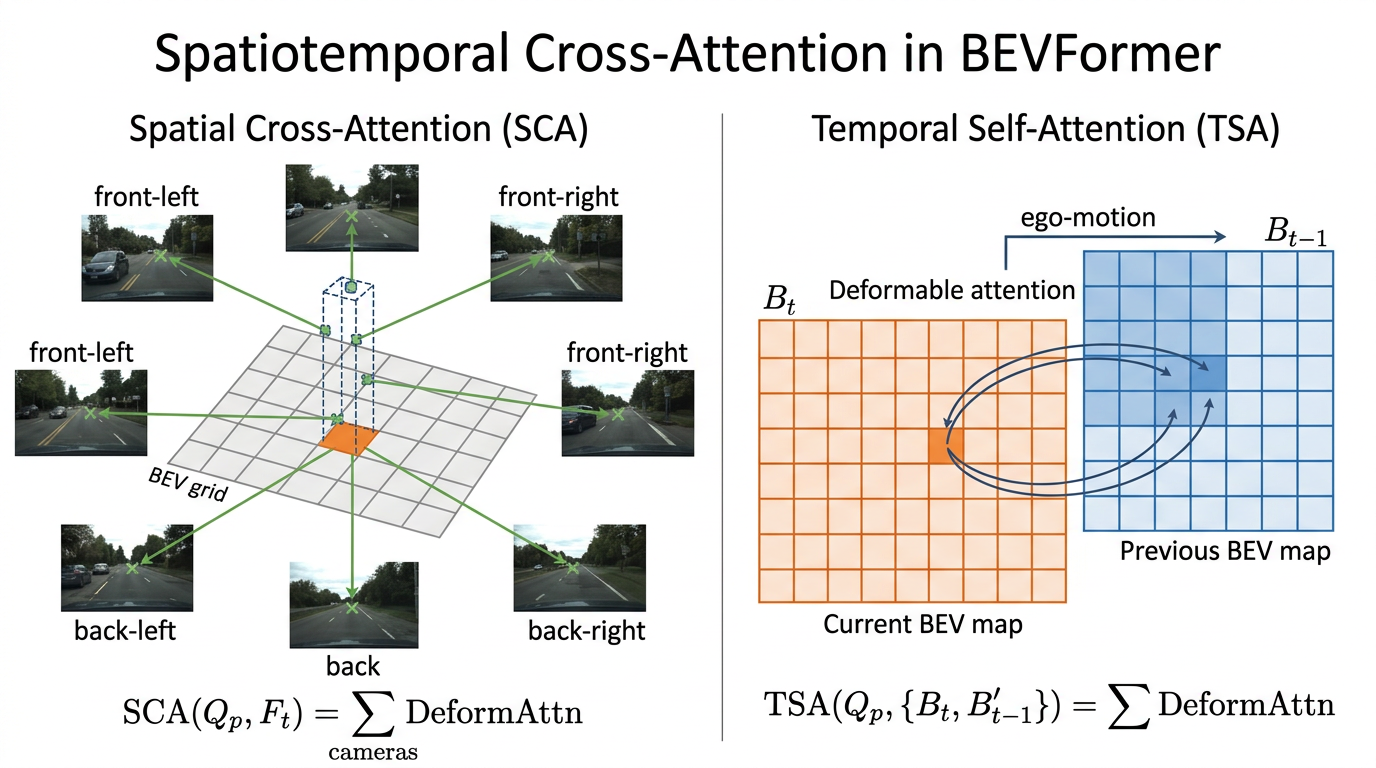
\includegraphics[width=\linewidth,keepaspectratio]{./figures/3D-Object-Detection-in-Autonomous-Driving__fig_mechanism.png}}
\caption{Spatiotemporal cross-attention mechanism in BEVFormer}\label{fig:fig-mechanism}\end{figure}

\subsection{Depth-Aware and Stereo Methods: BEVDepth, BEVStereo, MV-FCOS3D++}\label{depth-aware-and-stereo-methods-bevdepth-bevstereo-mv-fcos3d}

Depth supervision is the single most leveraged signal for closing the camera-LiDAR gap. BEVDepth \citep{li2023bevdepthacquisitio} realised that the implicit depth distribution learned by Lift-Splat-Shoot in BEVDet was the dominant source of error: although BEVDet's BEV-classification was strong, its depth was poorly calibrated, with mean error often exceeding 4 m at 60 m range. By projecting LiDAR ground truth onto the image plane and training the per-pixel depth distribution with explicit supervision, BEVDepth lifted nuScenes test NDS from 47.5\% to 60.0\% --- an 12.5-point absolute jump from a single auxiliary loss. BEVStereo \citep{li2023bevdepthacquisitio} further added temporal multi-view stereo: matching pixels across consecutive frames separated by ego-motion baseline gives geometric depth that can be triangulated, raising NDS by another 1--2 points and especially helping at range. BEVDet4D extended BEVDet with temporal warping. MV-FCOS3D++ \citep{wang2022detr3d3dobjectdete} extended FCOS3D to multi-view with pretrained monocular backbones, demonstrating Waymo-Camera-Only-Track competitive results.

Edge-Aware LSS (EA-LSS by Hu et al., 2023) added edge supervision to make the depth distribution sharper. SA-BEV \citep{zhang2023asimplebaselinefor} generated semantic-aware BEV features to handle the BEV foreground-background class imbalance. TiG-BEV \citep{huang2022monodtrmonocular3d} used target inner-geometry knowledge distillation from LiDAR teachers to camera-only students. UniDistill \citep{zhou2023unidistillaunivers} framed cross-modal distillation as a universal mechanism. \(X^3\)KD (Klingner et al., 2023) distilled across modalities, tasks, and stages.

The picture that emerges is that camera-only 3D detection has approximately tripled in NDS over four years --- from about 25 NDS in mid-2021 to about 70 NDS in mid-2024 --- almost entirely through better view transformation and explicit depth supervision. Yet a clear gap to LiDAR remains for distant and small targets: an 80 m pedestrian projects to \textasciitilde25 pixels in a 1600 × 900 nuScenes image, near the resolution limit, and depth ambiguity at such range can be 10 m or more. This is why camera-only systems are typically combined with high-definition map priors and aggressive temporal accumulation, and why production camera-only stacks (Tesla, Mobileye) emphasise dense occupancy prediction over sharp boxes.

\begin{table*}[t]
\centering
\caption{Depth-Aware and Stereo Methods: BEVDepth, BEVStereo, MV-FCOS3D++: comparative summary.}
\label{tab:depth-aware-and-stereo-methods-bevdepth-bevstereo-mv-fcos3d}
\begin{tabular}{>{\raggedright\arraybackslash}p{0.1667\linewidth}
  >{\raggedright\arraybackslash}p{0.0476\linewidth}
  >{\raggedright\arraybackslash}p{0.1905\linewidth}
  >{\raggedright\arraybackslash}p{0.2024\linewidth}
  >{\raggedright\arraybackslash}p{0.1905\linewidth}
  >{\raggedright\arraybackslash}p{0.0833\linewidth}
  >{\raggedright\arraybackslash}p{0.1190\linewidth}}
\toprule
Method & Year & Camera Setting & nuScenes Test NDS & nuScenes Val NDS & Latency & Backbone \\
\midrule
FCOS3D & 2021 & mono per-cam & 42.7\% (ens.) & 35.7\% & 80 ms & ResNet-101 \\
PGD & 2021 & mono & --- & 39.2\% & --- & ResNet-101 \\
DETR3D & 2022 & 6-cam queries & 47.9\% & 42.5\% & 200 ms & ResNet-101 \\
BEVDet & 2021 & LSS BEV & 48.8\% & 41.7\% & 100 ms & Swin-Tiny \\
BEVDet4D & 2022 & + temporal & 56.9\% & 51.5\% & 130 ms & Swin-Tiny \\
BEVFormer-S & 2022 & BEV cross-attn & 50.8\% & 47.6\% & 220 ms & ResNet-101 \\
BEVFormer-Base & 2022 & + temporal & 56.9\% & 51.7\% & 280 ms & ResNet-101 \\
PETR & 2022 & 3D pos enc & 50.4\% & 44.2\% & 220 ms & ResNet-101 \\
PETRv2 & 2022 & + temporal & 58.2\% & 52.4\% & 240 ms & VoVNet-99 \\
BEVDepth & 2023 & LSS + LiDAR sup. & 60.0\% & 53.5\% & 150 ms & ConvNeXt-B \\
BEVStereo & 2023 & + temp. stereo & 61.0\% & 54.6\% & 180 ms & ConvNeXt-B \\
Sparse4D v2 & 2023 & sparse recurrent & 71.4\% & 63.0\% & 160 ms & VoVNet-99 \\
Sparse4D v3 & 2023 & + det+track & 71.9\% & 65.6\% & 170 ms & VoVNet-99 \\
StreamPETR & 2023 & streaming & 67.6\% & 60.4\% & 160 ms & VoVNet-99 \\
Far3D & 2024 & 150 m surround & 63.5\% & 56.8\% & 200 ms & VoVNet-99 \\
RCBEVDet (R+C) & 2024 & radar+camera BEV & 56.6\% & 51.5\% & 140 ms & ResNet-50 \\
\end{tabular}
\end{table*}

Two patterns are visible. First, every step beyond the first-generation FCOS3D added temporal information: BEVDet4D, BEVFormer-temporal, PETRv2, BEVDepth (with adjacent-frame stereo), Sparse4D --- the consistent finding is that 3--5 historical frames add 5--10 NDS points by both densifying small targets and constraining motion. Second, sparse query detection has roughly closed the gap with multi-modal fusion: Sparse4D v3 at 71.9\% NDS is within 1 NDS point of BEVFusion at 72.9\%, and at lower latency. This is the most important shift in camera-only 3D detection of the 2023--2024 period and the one most likely to inform future deployment.

A practical limitation of all camera-only systems is the catastrophic effect of camera dropout. A single failed camera often costs 10--20 NDS points unless the detector has been explicitly trained with sensor dropout augmentation. This is one of the open robustness questions discussed in Section 9. The other practical limitation is calibration drift: a 0.5° rotational miscalibration on a 100 m target produces an 87 cm lateral error, which can change a ``merging'' object into a ``lane keeping'' object in a downstream tracker. Modern multi-camera detectors typically train on noisy calibration to be robust to small perturbations, but degradation from severe miscalibration remains a deployment hazard.

The next section synthesises the cross-modal fusion literature, where the strengths of LiDAR's metric depth meet the strengths of camera's dense semantics, and where the unified BEV representation has become the dominant integration substrate.
\section{Multi-Modal Fusion: LiDAR-Camera, Radar-Camera, and Beyond}\label{sec:multi-modal-fusion-lidar-camera-radar-camera-and-beyond}
Sensor fusion is, by any leaderboard measure, the highest-accuracy regime of 3D object detection. The state-of-the-art on the nuScenes test server has been held for over two years by multi-modal LiDAR-camera fusion methods such as BEVFusion (72.9\% NDS), TransFusion (71.7\%), and the cascading two-stage detectors that succeeded them. The intuition is direct: LiDAR provides metric depth and crisp geometric edges but lacks colour and fine-grained semantics, particularly at long range where its returns become extremely sparse; cameras provide dense colour and rich semantics but no depth. Radar, often a third modality, contributes velocity through Doppler and weather robustness. The two surveys that exhaustively organise this field are Wang et al.~(2023, IJCV) ``Multi-Modal 3D Object Detection in Autonomous Driving: A Survey'' and Wang, Zhang, Song et al.~(2023, IEEE TIV) ``Multi-Modal 3D Object Detection in Autonomous Driving: A Survey and Taxonomy''. Following their organisation, we group methods by the locus at which fusion happens --- input level, feature level, decision level --- and we add the increasingly important radar-camera and 4D-radar-LiDAR streams.

\subsection{Input-Level and Decoration Fusion: PointPainting, MVP}\label{input-level-and-decoration-fusion-pointpainting-mvp}

Input-level fusion is the simplest form: image semantic predictions are projected onto the LiDAR sweep so that each LiDAR point is ``painted'' with extra channels representing the image evidence at the projected pixel. PointPainting \citep{vora2020pointpaintingseque} was the canonical example. A 2D semantic-segmentation network --- e.g., DeepLab or HRNet trained on nuScenes-Image --- produced per-pixel class probabilities; for each LiDAR point, the projected pixel's class probability vector was concatenated to the point's \texttt{(x,\ y,\ z,\ r)} features; the resulting 4 + C-channel point cloud was fed unchanged to any downstream LiDAR detector (PointPillars, CenterPoint, PV-RCNN, etc.). This required no architectural change, added 2--4 ms of overhead, and on nuScenes typically yielded 3--6 NDS points over the LiDAR-only baseline. Multimodal Virtual Point (MVP, Yin, Zhou, and Krähenbühl, 2021) generalised this by inserting ``virtual'' 3D points sampled from image-derived dense depth around foreground regions, densifying sparse LiDAR by an order of magnitude on small distant objects and improving small-class AP by 5--15 points.

The strengths of input-level fusion are clarity, modularity, and the fact that any LiDAR detector benefits without retraining its core backbone. The weaknesses are the dependence on a separate, pre-trained 2D semantic network --- which adds 50--100 ms of latency and consumes its own memory --- and the fragility under camera failure, since the painted channels become noisy when one camera drops out. PointPainting and MVP are still strong baselines and frequently appear as components of cascaded detectors.

\subsection{Feature-Level BEV Fusion: BEVFusion, DeepFusion, FUTR3D, TransFusion}\label{feature-level-bev-fusion-bevfusion-deepfusion-futr3d-transfusion}

The dominant fusion family today is feature-level fusion in the bird's-eye-view representation. BEVFusion (Liu, Tang, Amini et al., 2022; ICRA 2023, \textasciitilde960 citations) was the breakthrough: rather than projecting either modality into the other's representation, it transformed both into a common BEV grid. The LiDAR branch followed a standard sparse 3D convolution backbone (CenterPoint-style) producing a BEV feature \texttt{\$B\_L\$\ ∈\ \$R\^{}\{C\ ×\ 200\ ×\ 200\}$}. The camera branch followed a Lift-Splat-Shoot view-transform with explicit depth estimation, producing \texttt{$B\_C\$\ ∈\ \$R\^{}\{C\ ×\ 200\ ×\ 200\}\$} over the same metric grid. The two BEV tensors were concatenated, fed through a fused BEV CNN, and decoded by a CenterPoint-style head. BEVFusion reached 72.9\% NDS on the nuScenes test server, exceeding any LiDAR-only or camera-only baseline by a wide margin, and became the architecture against which all subsequent fusion detectors compare.

TransFusion adopted a different fusion locus: query-based decoding with two stages of cross-attention. A first stage of object queries cross-attended to LiDAR features producing initial proposals; a second stage cross-attended to image features to refine. TransFusion reached 71.7\% NDS. FUTR3D (Chen, Zhang, Wang et al., 2023; CVPR Workshops) presented a sensor-agnostic decoder that consumed any combination of LiDAR, camera, and radar through a shared modal-agnostic transformer; it reached 68.3\% NDS with all three modalities active. DeepFusion \citep{li2022bevformerlearningb} cross-attended camera features into LiDAR features at the voxel level rather than the BEV level. EPNet++ (Liu, Huang, Li et al., 2022; PAMI) used cascade bi-directional fusion blocks that exchanged information between LiDAR and image branches at multiple scales. PI-RCNN (Xie, Xiang, Yu et al., 2020) fused via point-based attentive cont-conv. PointAugmenting and Frustum PointPillars are earlier methods of the same family.

A more recent direction is sparse fusion. SparseFusion (Xie, Xu, Rakotosaona et al., 2023; ICCV) operated entirely on sparse representations on both sides --- sparse LiDAR queries and sparse image queries --- and reached 73.9\% NDS at lower latency than dense BEV. Fully Sparse Fusion \citep{li2023bevdepthacquisitio} extended this to long-range scenarios where dense BEV becomes prohibitive. LoGoNet \citep{li2023bevdepthacquisitio} added local-to-global cross-modal fusion blocks. UniDistill (Zhou, Liu, Hu et al., 2023; CVPR) framed cross-modal knowledge distillation as a universal mechanism, training a camera-only student from a LiDAR teacher and recovering 4--8 NDS points. Dense Voxel Fusion (Mahmoud, Hu, and Waslander, 2023; WACV) fused at the voxel level with dense camera features projected through depth. SimpleBEV (Zhao et al., 2024) demonstrated an even simpler fusion architecture matching BEVFusion at lower complexity. CL-fusionBEV (Shi et al., 2024) unified camera-LiDAR fusion in BEV. M3Net (Chen et al., 2025) extended multi-modal fusion to multi-task: detection, segmentation, and occupancy in a single network. MV2DFusion (Wang et al., 2026, PAMI) leveraged modality-specific object semantics for multi-modal 3D detection.

BiCo-Fusion \citep{song2024robustnessaware3do} introduced bidirectional complementary LiDAR-camera fusion explicitly designed to be both semantic- and spatial-aware. CIDRA-Net (Yu et al., 2025) added cross-modal interaction with distribution-relation awareness, addressing the implicit assumption that LiDAR and camera distributions are statistically aligned. AEPF (Sharma et al., 2024) introduced attention-enabled point fusion. PVAFN \citep{li2024bevformerlearningb} combined point-voxel attention with multi-pooling, extending the hybrid family with explicit cross-modal queries.

\subsection{Radar-Camera and 4D Radar Fusion: RADIANT, RCBEVDet, L4DR}\label{radar-camera-and-4d-radar-fusion-radiant-rcbevdet-l4dr}

Radar fusion has historically been under-explored relative to LiDAR-camera, in part because traditional 3D radar is extremely sparse and its azimuth resolution (1--3°) is poor compared with LiDAR (0.08--0.35°). The recent appearance of 4D imaging radar --- which adds elevation through a virtual MIMO array --- has changed the calculus, producing roughly 1,000--10,000 points per scan with native range, Doppler, and azimuth-elevation. RADIANT (Long, Kumar, Morris et al., 2023; AAAI) used radar as a depth oracle for monocular 3D detection: it associated radar detections with 2D image proposals through a learned association network and used the radar range to disambiguate the depth of monocular boxes, reducing depth error on cars from a mean of 4.2 m to 1.8 m. RCBEVDet (Lin, Liu, Xia et al., 2024; CVPR) integrated radar BEV with camera BEV through cross-modal attention and reached 56.6\% NDS on nuScenes test, a 5--8 NDS improvement over the camera-only BEVDet baseline. ClusterFusion (Kurniawan and Trilaksono, 2023) pre-clustered radar points to enrich each cluster with camera context. CRN (Camera Radar Net) achieved 62.4\% NDS through transformer-based cross-modal attention. RCM-Fusion is a more recent variant.

LiDAR-radar fusion is still nascent. L4DR \citep{huang2024l4drlidar4dradarfu} fused 4D imaging radar with LiDAR and demonstrated weather-robust 3D detection: under heavy fog (visibility \textless{} 50 m) the LiDAR-only baseline lost roughly 25 mAP, while L4DR recovered the loss to within 5 mAP of clear weather, vindicating the long-standing argument that radar should be the third sensor in safety-critical perception.

The radar-camera and LiDAR-radar lines are particularly important for ADAS deployments, where LiDAR is too expensive, but a single camera is too brittle. The best recent radar-camera systems on nuScenes lag the best LiDAR-camera systems by roughly 12--16 NDS points but are within 1--3 NDS of camera-only and at significantly lower BOM cost.

\subsection{Comparative summary}\label{comparative-summary}

A few cross-cutting observations are worth flagging. First, the dominant fusion locus has migrated upward over five years: from input-level decoration (PointPainting, 2020) to feature-level BEV (BEVFusion, 2022) to sparse query (SparseFusion, 2023) to multi-task multi-modal (M3Net, 2025). Each step has typically added 2--4 NDS points on nuScenes while reducing or holding latency constant. Second, the gap between multi-modal fusion and well-designed camera-only systems has narrowed sharply, from 27 NDS points (BEVFusion 72.9\% vs DETR3D 47.9\% in 2022) to roughly 1 NDS point (BEVFusion 72.9\% vs Sparse4D v3 71.9\% in 2023). Third, robustness benchmarks (MultiCorrupt, L4DR) have surfaced an uncomfortable finding: many LiDAR-camera fusion methods rely heavily on the camera under nominal conditions but degrade more than expected when the camera fails --- sometimes worse than a LiDAR-only baseline. This robustness asymmetry is now driving research into modality-balanced training and modality dropout regularisation.

\begin{table*}[t]
\centering
\caption{Comparative summary: comparative summary.}
\label{tab:comparative-summary}
\begin{tabular}{>{\raggedright\arraybackslash}p{0.1566\linewidth}
  >{\raggedright\arraybackslash}p{0.0482\linewidth}
  >{\raggedright\arraybackslash}p{0.2410\linewidth}
  >{\raggedright\arraybackslash}p{0.2048\linewidth}
  >{\raggedright\arraybackslash}p{0.0843\linewidth}
  >{\raggedright\arraybackslash}p{0.2651\linewidth}}
\toprule
Method & Year & Modalities & nuScenes Test NDS & Latency & Notes \\
\midrule
PointPainting & 2020 & L + C (input) & 58.1\% & +50 ms & trivial overlay \\
MVP & 2021 & L + C (virtual pts) & 70.5\% & +120 ms & small-class focus \\
3D-CVF & 2020 & L + C (cross-view) & 65.7\% & 130 ms & feature fusion \\
EPNet++ & 2022 & L + C (cascade) & 64.0\% & 150 ms & bi-directional \\
DeepFusion & 2022 & L + C (voxel) & 70.7\% & 110 ms & InverseAug \\
TransFusion & 2022 & L + C (query) & 71.7\% & 140 ms & two-stage \\
BEVFusion & 2022 & L + C (BEV) & 72.9\% & 120 ms & unified BEV \\
FUTR3D & 2023 & L + C (+R) & 68.3\% & 180 ms & sensor-agnostic \\
SparseFusion & 2023 & L + C (sparse) & 73.9\% & 100 ms & fully sparse \\
LoGoNet & 2023 & L + C (local-global) & 73.5\% & 130 ms & KITTI-strong \\
UniDistill & 2023 & KD L→C & 64.6\% & 80 ms & camera-only deployment \\
MV2DFusion & 2026 & L + C (semantics) & 75.0\% & 130 ms & latest TPAMI \\
RADIANT & 2023 & C + R & 47.4\% & 90 ms & radar depth oracle \\
RCBEVDet & 2024 & C + R (BEV) & 56.6\% & 140 ms & radar BEV fusion \\
CRN & 2023 & C + R & 62.4\% & 130 ms & xModal attention \\
L4DR & 2024 & L + 4D-R & 71.4\% & 160 ms & weather robust \\
Snow-CLOCs & 2024 & L + C (decision) & 67.0\% & 110 ms & snow-focused \\
\end{tabular}
\end{table*}

Across this tabulation, three takeaways crystallise. The unified BEV representation is the de facto fusion substrate. Sparse query designs are catching up on accuracy while being faster, suggesting they are likely to be the deployment-friendly choice. And radar --- both 3D and 4D --- is the hedge against weather and camera-only failure that the field has under-invested in for nearly a decade. The next section addresses cooperative perception, where the fusion is across vehicles rather than across sensors on a single ego.
\section{Cooperative V2X 3D Object Detection}\label{sec:cooperative-v2x-3d-object-detection}
A single ego vehicle, no matter how richly instrumented, has fundamental perceptual blind spots: it cannot see around an opaque parked truck, around a building corner at an unsignalised intersection, or beyond the 120 m reliable range of its onboard 32-beam LiDAR. Cooperative perception --- also known as Vehicle-to-Everything (V2X), Vehicle-to-Vehicle (V2V), and Vehicle-to-Infrastructure (V2I) perception --- addresses this through wireless communication that lets vehicles and roadside units (RSUs) exchange perception data and merge them into a shared 3D scene. This section reviews the datasets that enabled the field, the architectures that exchange features rather than raw points or final boxes, and the bandwidth-latency-accuracy trade-offs that determine deployability. The exhaustive references for this section are the F-Cooper paper of Chen et al.~(2019, ACM/IEEE SEC, \textasciitilde382 citations), the V2X-ViT family of Xu et al.~(2022 ECCV, 2024 PAMI), the DAIR-V2X dataset of Yu et al.~(2022, CVPR), and the FFNet feature-flow papers of Yu, Tang, Xie et al.~(2023).

\subsection{Datasets and Communication Constraints: DAIR-V2X, OPV2V, V2X-Set}\label{datasets-and-communication-constraints-dair-v2x-opv2v-v2x-set}

The cooperative perception subfield emerged in 2019 but only became mature when public datasets appeared. DAIR-V2X (Yu, Luo, Shu et al., 2022; CVPR) was the first large-scale real-world cooperative dataset, providing approximately 71,254 pairs of synchronized vehicle and infrastructure sensor data --- collected by an autonomous test vehicle and a fixed roadside LiDAR + camera unit at intersections in Beijing --- with 3D box annotations on both sides. DAIR-V2X-V (vehicle), DAIR-V2X-I (infrastructure), and DAIR-V2X-C (cooperative) sub-tracks isolate the gain attributable to the cooperative signal. OPV2V (Open Perception V2V) is a simulator-based V2V dataset built in CARLA with up to seven connected vehicles per scene; its training set covers 73 scenes and 11,464 frames. V2X-Set is a more recent simulation dataset designed specifically for benchmarking V2X-ViT-style transformers. CoopDet3D, V2V4Real, and Rope3D (the largest roadside dataset, with over 50,000 manually annotated frames in 1080p with 4D box labels) round out the public landscape. Tumtraf-V2X provides a real-world dataset from German intersections.

Communication constraints define the achievable accuracy. The C-V2X PC5 sidelink at 5.9 GHz provides \textasciitilde10 Mbps in dense urban deployment with end-to-end latency of 30--100 ms; DSRC (IEEE 802.11p) provides \textasciitilde6 Mbps with similar latency. Sharing raw LiDAR points (\textasciitilde1 MB/sweep at 10 Hz = 10 Mbps after compression) saturates these links and incurs unacceptable end-to-end latency, while sharing only final boxes (a few hundred bytes/frame) loses most of the cooperative signal. The architectural sweet spot --- and the focus of essentially all post-2020 work --- is the exchange of intermediate BEV feature maps with adaptive compression.

\subsection{Cooperative Architectures: F-Cooper, V2X-ViT, FFNet, V2X-ViTv2}\label{cooperative-architectures-f-cooper-v2x-vit-ffnet-v2x-vitv2}

F-Cooper (Chen, Ma, Tang et al., 2019; ACM/IEEE SEC) was the first deep cooperative perception system. Each connected vehicle ran its own VoxelNet detector up to the BEV feature stage, broadcast its compressed BEV feature map together with its global pose, and used a max-pooling fusion at receivers after warping the received feature into the receiver's frame using the pose offset. F-Cooper improved AP at distant occluded targets by 20--30 percentage points relative to non-cooperative baselines on a CARLA evaluation, demonstrating that the dominant value of cooperation is around occluded and corner cases.

V2X-ViT (Xu, Xiang, Tu et al., 2022; ECCV) generalised this with a transformer-based fusion that explicitly modelled (a) the heterogeneity between vehicle-mounted and infrastructure-mounted sensors, which often have different beam patterns, mounting heights, and time bases, and (b) the spatial misalignment caused by GPS error and clock skew. The Heterogeneous Multi-Agent Self-Attention (HMSA) and Multi-Scale Window Attention (MSwin) modules of V2X-ViT achieved 71.4\% AP on V2X-Set under the IoU 0.5 threshold and 67.9\% AP on the more difficult OPV2V cross-domain evaluation. V2X-ViTv2 (Xu, Chen, Tu et al., 2024; PAMI) extended the framework with improved transformer designs and consistent gains across simulation and real-world cooperative datasets.

FFNet \citep{yu2023vehicleinfrastruct} addressed the latency problem head-on through Feature-Flow Prediction. Because the wireless link introduces 30--100 ms of delay between the moment an infrastructure sensor captures a frame and the moment a vehicle can use it, naive fusion combines stale infrastructure features with current ego features. FFNet learned to predict the optical-flow-style displacement of BEV features from \texttt{t−Δt} to \texttt{t} so that the warped features could be fused with the current ego BEV without staleness. The accompanying paper ``Vehicle-Infrastructure Cooperative 3D Object Detection via Feature Flow Prediction'' reported a 4--7 mAP gain at typical realistic 100 ms latencies on DAIR-V2X compared with a no-flow baseline. ViT-FuseNet \citep{zhou2023unidistillaunivers} extended the multi-modal V2X fusion to combine roadside vision-transformer image features with vehicle-side LiDAR features. CoFormerNet \citep{li2024bevformerlearningb} built a transformer fusion approach explicitly for vehicle-infrastructure cooperative perception. Calibration-Free BEV Representation (Fan et al., 2023, IROS) addressed the under-appreciated reality that infrastructure cameras' intrinsic and extrinsic calibration drifts over time, and proposed a calibration-free BEV that could absorb up to 5° of rotational miscalibration.

InfraDet3D (Zimmer et al., 2023) is a roadside-only system fusing camera and LiDAR at intersection RSUs. MIC-BEV \citep{zhang2025anewliteraturerevi} extended infrastructure-camera-only BEV detection with relation-aware transformer fusion. BEVHeight++ \citep{yang2023bevheighttowardrob} is a vision-centric infrastructure detector that uses height regression rather than depth regression to be more robust to mounting-angle perturbation. Cross-Domain Generalization (Zhi et al., 2025) studied the generalisation gap between vehicle and infrastructure environments, finding that infrastructure sensors typically have much narrower viewpoint distributions than vehicles, making cross-environment generalisation more difficult than the same-environment case.

\subsection{Latency and Bandwidth Trade-offs in Vehicle-Infrastructure Cooperation}\label{latency-and-bandwidth-trade-offs-in-vehicle-infrastructure-cooperation}

The deployment of cooperative perception ultimately turns on three jointly optimised quantities: bandwidth (bytes per agent per second exchanged), latency (end-to-end from sensor capture on agent A to detection delivery on agent B), and detection accuracy (AP at a given IoU threshold). Three operating points are commonly distinguished. Early fusion exchanges raw point clouds: bandwidth is high (10 Mbps per agent) but accuracy is highest because no local preprocessing has destroyed information. Intermediate fusion exchanges BEV feature maps after local processing: bandwidth drops to roughly 0.3--1.0 Mbps per agent with adaptive compression and accuracy is within 2--4 mAP of early fusion in the standard regime. Late fusion exchanges only final boxes: bandwidth is negligible (\textless10 kbps) but accuracy is 5--10 mAP lower because spatial overlap and uncertainty information are discarded. The DAIR-V2X benchmark explicitly measures ``Latency-AP'', which evaluates accuracy as a function of communication latency. FFNet, by predicting the feature flow, dominates this curve at 50--200 ms latency.

Privacy and security are the underexplored axes. Sharing raw camera feeds raises GDPR-style concerns; sharing BEV features is more palatable but still encodes recoverable visual information. Cross-Modal Phantom (Khan and Hasan, 2026) demonstrated that coordinated camera-LiDAR spoofing attacks can fool multi-sensor fusion stacks, raising the broader question of whether cooperative perception's added trust assumptions create new attack surfaces. Authentication of the V2X identity, encrypted feature exchange, and Byzantine-robust fusion are all active research questions.

\begin{table*}[t]
\centering
\caption{Latency and Bandwidth Trade-offs in Vehicle-Infrastructure Cooperation: comparative summary.}
\label{tab:latency-and-bandwidth-trade-offs-in-vehicle-infrastructure-c}
\begin{tabular}{>{\raggedright\arraybackslash}p{0.1556\linewidth}
  >{\raggedright\arraybackslash}p{0.0444\linewidth}
  >{\raggedright\arraybackslash}p{0.2667\linewidth}
  >{\raggedright\arraybackslash}p{0.1333\linewidth}
  >{\raggedright\arraybackslash}p{0.1000\linewidth}
  >{\raggedright\arraybackslash}p{0.1889\linewidth}
  >{\raggedright\arraybackslash}p{0.1111\linewidth}}
\toprule
System & Year & Modality & Dataset & Bandwidth & Latency Tolerance & AP@IoU 0.5 \\
\midrule
F-Cooper & 2019 & LiDAR BEV feature & CARLA-3 cars & \textasciitilde0.5 Mbps & \textasciitilde30 ms & 64.0\% \\
AttFuse & 2022 & LiDAR BEV + attention & OPV2V & \textasciitilde0.5 Mbps & \textasciitilde50 ms & 73.5\% \\
V2X-ViT & 2022 & LiDAR BEV transformer & V2X-Set & \textasciitilde0.4 Mbps & \textasciitilde100 ms & 71.4\% \\
V2X-ViTv2 & 2024 & LiDAR BEV transformer v2 & OPV2V & \textasciitilde0.4 Mbps & \textasciitilde100 ms & 75.1\% \\
FFNet & 2023 & LiDAR + flow predict & DAIR-V2X-C & \textasciitilde0.3 Mbps & up to 200 ms & 70.7\% \\
Where2Comm & 2022 & adaptive BEV mask & OPV2V & adaptive & \textasciitilde80 ms & 73.4\% \\
CoFormerNet & 2024 & multi-modal V2I & DAIR-V2X & \textasciitilde0.6 Mbps & \textasciitilde80 ms & 69.8\% \\
InfraDet3D & 2023 & roadside L+C & private & ego-only & n/a & 65.4\% \\
BEVHeight++ & 2023 & infrastructure cam & DAIR-V2X-I & \textasciitilde0.2 Mbps & \textasciitilde50 ms & 56.6\% \\
Calib-Free BEV & 2023 & infrastructure cam & DAIR-V2X-I & \textasciitilde0.2 Mbps & \textasciitilde50 ms & 53.4\% \\
\end{tabular}
\end{table*}

The cumulative pattern is that 70--75\% AP on V2X benchmarks is achievable at realistic 100 ms latencies and sub-megabit bandwidth budgets. The fundamental gain from cooperative perception is concentrated in the long tail of occluded and out-of-range targets --- exactly the targets that most contribute to safety-critical edge cases. This makes cooperative perception arguably the highest-leverage open research direction in autonomous driving for the late 2020s, and explains the recent push by Chinese OEMs (Baidu, Huawei, China Mobile) toward standardised C-V2X-based intelligent transportation systems and the Tier-1 deployment of V2X-ready RSUs in pilot cities.

A practical limitation is that V2X is, by definition, a network effect: one V2X-equipped vehicle is useless without partners. Production deployments therefore require coordinated rollouts of vehicle-side and infrastructure-side hardware, which has historically lagged behind the algorithmic state of the art by 5--10 years. The most plausible near-term deployment is V2I in geofenced commercial corridors (logistics centres, ports, airports, ride-share staging zones) where infrastructure can be installed once and amortised across a controlled fleet. The robotaxi segment of Waymo and Cruise has so far avoided V2X dependence, betting that improved on-board perception and high-definition maps make the cooperative gain marginal in their operational design domain. The truth probably lies in between: cooperative perception is essential for unprotected dense urban driving, optional elsewhere.

The next section examines the datasets and metrics that have made all of the comparisons in this and earlier sections possible, and makes their numerical specifications explicit at the level of detail required to interpret leaderboard results.
\section{Datasets, Benchmarks, and Evaluation Metrics}\label{sec:datasets-benchmarks-and-evaluation-metrics}
The choice of dataset and metric controls more of the apparent state-of-the-art ranking than any single architectural change. A camera-only detector that ranks first on KITTI may rank fifth on nuScenes, because KITTI emphasises tightly cropped front-facing scenes with abundant 64-beam LiDAR ground-truth, while nuScenes emphasises 360° surround coverage and small/distant objects. Reading a leaderboard correctly requires knowing exactly what the dataset measures, what the metric rewards, and what the typical confidence interval on each score is. This section provides those concrete numerical specifications.

\subsection{KITTI, nuScenes, Waymo Open Dataset, Argoverse 2 in Detail}\label{kitti-nuscenes-waymo-open-dataset-argoverse-2-in-detail}

\textbf{KITTI} \citep{geiger2012arewereadyforauton} is the original benchmark and remains the entry point for most academic 3D detection. The 3D Object Detection split contains 7,481 training images and 7,518 test images, collected with a Velodyne HDL-64E LiDAR (64 beams, 26.9° vertical, 0.08° horizontal), four cameras (two greyscale stereo and two colour stereo at 1242 × 375), and a high-precision IMU/GPS, in five environments around Karlsruhe, Germany. There are roughly 80,000 3D bounding boxes labelled across three primary classes --- Car, Pedestrian, Cyclist --- split into Easy / Moderate / Hard difficulty bands by occlusion and truncation. The official metric is 3D AP at IoU 0.7 (cars) and IoU 0.5 (pedestrians, cyclists), aggregated over 11 (legacy) or 40 (current) recall positions. Annotated objects are limited to the front-facing camera frustum within \textasciitilde70 m, which makes KITTI a poor proxy for full surround-view modern driving.

\textbf{nuScenes} \citep{caesar2020nuscenesamultimoda} is the dataset that most modern surround-view methods benchmark on. It comprises 1,000 driving sequences (850 trainval + 150 test) of 20 seconds each, recorded in Boston and Singapore, with key-frame annotations every 0.5 seconds. The sensor suite includes one 32-beam Velodyne HDL-32E LiDAR (10 Hz, 5°-vertical resolution), six 1600 × 900 cameras (12 Hz, \textasciitilde70° FoV each, mounted to give 360° coverage), five 77 GHz Continental ARS408-21 radars, and a GNSS-IMU. Annotations cover 23 categories with approximately 1.4 million 3D bounding boxes total. The official benchmark uses 10 detection classes (car, truck, construction vehicle, bus, trailer, barrier, motorcycle, bicycle, pedestrian, traffic cone). The unique feature of nuScenes is that it is the only major dataset with full radar coverage and per-instance velocity annotation. Total raw size is approximately 345 GB.

\textbf{Waymo Open Dataset (WOD)} Perception v1.4 (Sun et al., 2020) is the largest. It contains 1,150 driving segments of 20 seconds each (798 train + 202 val + 150 test), captured in Phoenix, Mountain View, San Francisco, and Kirkland, with one mid-range top-LiDAR plus four short-range LiDARs (5 LiDARs total, each \textasciitilde10 Hz) and five 1920 × 1280 cameras (one front + four perimeter). The dataset has approximately 12.6 million 3D box labels and 9.9 million 2D box labels across 200,000 frames sampled at 10 Hz. The detection classes are Vehicle, Pedestrian, Cyclist, Sign. The official metric is APH (heading-aware AP), which weights each true positive by its heading accuracy \texttt{\textbar{}cos(Δθ)\textbar{}}, severely penalising 180° errors. Levels L1 and L2 partition the difficulty by point density: L1 includes objects with ≥5 LiDAR points, L2 includes ≥1 point. Camera-only evaluation uses LET-3D-AP \citep{hung2022let3daplongitudina}, a longitudinal-error tolerant variant that allows camera-only detectors to score reasonably despite their depth ambiguity.

\textbf{Argoverse 2} (Wilson et al., 2023) provides 1,000 logs at 20 Hz with 26 detection categories, including long-tail classes such as \texttt{\$school\_b\$us}, \texttt{wheelchair}, and \texttt{stroller}. Argoverse and Argoverse 2 are notable for offering rich HD-map priors paired with detection, which is increasingly relevant as map-aware detectors become standard.

\textbf{A*3D} (Pham, Sevestre, Pahwa et al., 2019) was an early dataset focused on challenging environments --- heavy rain, low light --- with 39,179 frames. \textbf{ApolloScape} is Baidu's large urban-driving dataset. \textbf{ONCE} (One Million Scenes) is a Chinese dataset of one million LiDAR sweeps, used primarily for self-supervised pre-training. \textbf{DAIR-V2X} and \textbf{OPV2V} are the cooperative-perception datasets discussed in Section 7. The Lyft Level 5 Perception Dataset, since acquired by Woven Planet, contains 1,118 scenes of urban driving in Palo Alto.

\begin{figure}[t]
\centering
\pandocbounded{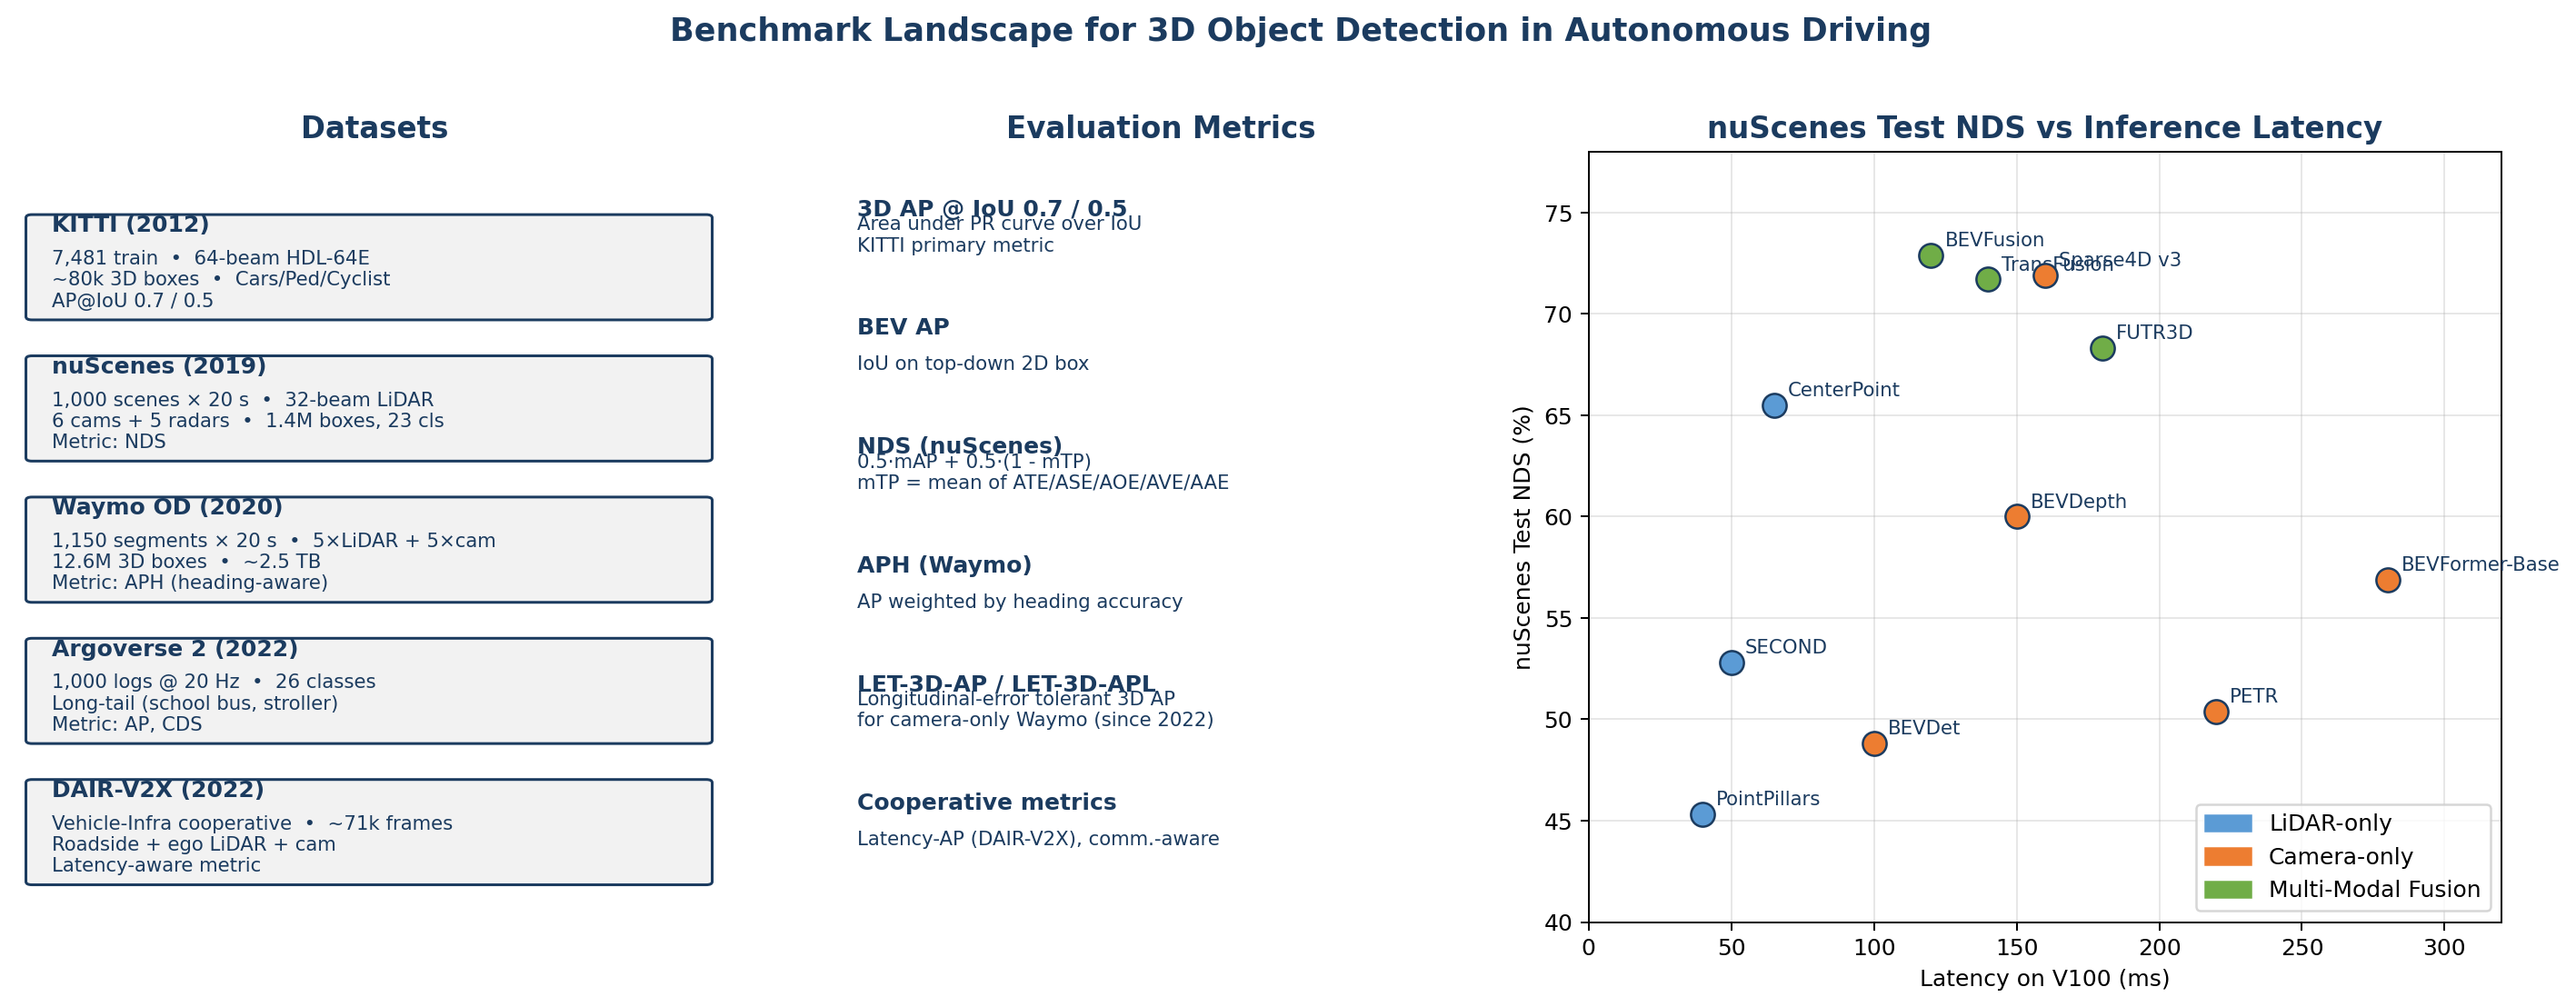
\includegraphics[width=\linewidth,keepaspectratio]{./figures/3D-Object-Detection-in-Autonomous-Driving__fig_benchmarks.png}}
\caption{Benchmark landscape for 3D object detection}\label{fig:fig-benchmarks}\end{figure}

\subsection{Evaluation Metrics: 3D AP, NDS, APH, LET-3D-AP}\label{evaluation-metrics-3d-ap-nds-aph-let-3d-ap}

The metric most familiar to the field is \textbf{3D AP}: a true positive requires the predicted 3D box to overlap a ground-truth box with IoU above a threshold (0.7 for cars on KITTI, 0.5 for pedestrians/cyclists), and the precision-recall curve is integrated. The 3D IoU between two oriented cuboids is computed by intersecting their BEV projections --- a polygon-polygon clip --- and multiplying by the height-overlap fraction; this is non-trivial to implement correctly and small numerical differences in the IoU implementation can swing a published number by 0.5--1 AP. \textbf{BEV AP} uses 2D IoU on the BEV projection only, and is typically \textasciitilde5 AP higher than 3D AP because height errors no longer count.

\textbf{nuScenes Detection Score (NDS)} is a composite metric that combines mAP across 10 classes at four distance-based IoU thresholds with five mean true-positive errors. Specifically, NDS = \texttt{0.5\ ·\ mAP\ +\ 0.5\ ·\ (1\ −\ mTP)}, where \texttt{mTP} is the mean of mATE (Average Translation Error in metres), mASE (Average Scale Error), mAOE (Average Orientation Error in radians), mAVE (Average Velocity Error in m/s, computed only on classes with annotated velocity), and mAAE (Average Attribute Error). Each error is normalised to {[}0, 1{]} before averaging. NDS is bounded in {[}0, 1{]} and reported in percentage. The motivation is that a metric that rewards both detection rate and localisation precision better captures driving-relevant performance than mAP alone.

\textbf{APH (Waymo)} weights each true positive by \texttt{\textbar{}cos(Δθ)\textbar{}} where \texttt{Δθ} is the heading angle error, severely penalising heading flips. Waymo also reports L1 and L2 versions for different difficulty regimes. \textbf{LET-3D-AP} and \textbf{LET-3D-APL} \citep{hung2022let3daplongitudina} tolerate longitudinal errors up to 10--20\% of the depth, which is the ratio at which depth ambiguity becomes geometrically irreducible for monocular cameras; this metric is the recommended one for camera-only Waymo evaluation since 2022.

A growing concern is that detection metrics do not capture downstream driving behaviour. A box localisation error of 0.5 m on a parked car at 50 m has near-zero safety consequence; the same error on a moving pedestrian at 10 m is potentially catastrophic. Planner-aware metrics such as PKL (Planner KL-divergence) and L4 metrics that condition on collision-relevance are early efforts in this direction but have not yet been widely adopted. The 2026 BEV survey-of-surveys (Li, Zhao, Zhong et al., IEEE TITS) argues for safety-relevance reweighting as the next step in metric design.

\subsection{Reproducibility and Leaderboard Snapshots}\label{reproducibility-and-leaderboard-snapshots}

To make leaderboard results comparable, modern publications typically include the following information: backbone choice and parameter count, image resolution and aug, point-cloud frame count (single-sweep versus multi-sweep, e.g., 10 sweeps for nuScenes), training schedule (often the ``1×'' of 12 epochs versus ``2×'' of 24), and test-time augmentation (TTA) strategy. Failing to control for these makes year-on-year comparison meaningless. For example, BEVFusion-Camera reaches 53.5\% NDS without TTA and 60.6\% with multi-scale TTA --- a 7-NDS-point swing from a single hyperparameter.

A representative snapshot of the nuScenes test leaderboard, as it commonly appears in 2024 papers, is shown below. Latency figures are approximate, on a single Tesla V100, with batch size 1 and FP32 inference unless otherwise noted; INT8 deployment can halve these numbers.

\begin{table*}[t]
\centering
\caption{Reproducibility and Leaderboard Snapshots: comparative summary.}
\label{tab:reproducibility-and-leaderboard-snapshots}
\begin{tabular}{>{\raggedright\arraybackslash}p{0.1739\linewidth}
  >{\raggedright\arraybackslash}p{0.1159\linewidth}
  >{\raggedright\arraybackslash}p{0.1449\linewidth}
  >{\raggedright\arraybackslash}p{0.2464\linewidth}
  >{\raggedright\arraybackslash}p{0.0725\linewidth}
  >{\raggedright\arraybackslash}p{0.0725\linewidth}
  >{\raggedright\arraybackslash}p{0.0725\linewidth}
  >{\raggedright\arraybackslash}p{0.1014\linewidth}}
\toprule
Method & Modality & Backbone & nuScenes Test NDS & mAP & mATE & mAVE & Latency \\
\midrule
PointPillars & LiDAR & -- & 45.3\% & 30.5\% & 0.517 & 0.316 & 16 ms \\
SECOND & LiDAR & SparseConv & 52.8\% & 41.4\% & 0.426 & 0.292 & 50 ms \\
CenterPoint & LiDAR & VoxelNet & 65.5\% & 58.0\% & 0.305 & 0.285 & 65 ms \\
AFDetV2 & LiDAR & SparseConv & 68.7\% & 62.4\% & 0.282 & 0.235 & 70 ms \\
FCOS3D & Camera & ResNet-101 & 42.7\% (ens.) & 35.8\% & 0.690 & 1.434 & 80 ms \\
DETR3D & Camera & ResNet-101 & 47.9\% & 41.2\% & 0.641 & 0.845 & 200 ms \\
BEVFormer-B & Camera & ResNet-101 & 56.9\% & 48.1\% & 0.582 & 0.378 & 280 ms \\
BEVDepth & Camera & ConvNeXt-B & 60.0\% & 52.0\% & 0.450 & 0.262 & 150 ms \\
Sparse4D v3 & Camera & VoVNet-99 & 71.9\% & 65.6\% & 0.437 & 0.225 & 170 ms \\
TransFusion & L+C & -- & 71.7\% & 68.9\% & 0.259 & 0.258 & 140 ms \\
BEVFusion & L+C & -- & 72.9\% & 70.2\% & 0.254 & 0.254 & 120 ms \\
SparseFusion & L+C & -- & 73.9\% & 70.4\% & 0.235 & 0.243 & 100 ms \\
MV2DFusion & L+C & -- & 75.0\% & 70.5\% & 0.232 & 0.224 & 130 ms \\
RCBEVDet & C+R & ResNet-50 & 56.6\% & 45.3\% & 0.486 & 0.245 & 140 ms \\
\end{tabular}
\end{table*}

Beyond the headline numbers, several robustness scores have started to matter: multi-frame consistency (whether the same object is detected in consecutive frames at a stable identity), long-range AP (typically computed at 50--80 m and 80--150 m bins), and rare-class recall. Argoverse 2's scoring explicitly weights long-tail classes more heavily through a category-balanced metric.

The reproducibility crisis that has affected other areas of computer vision is partially mitigated in 3D detection by the existence of the OpenPCDet library (PV-RCNN, CenterPoint, PointPillars, Voxel R-CNN, Voxel Set Transformer), the MMDetection3D framework, and the Detectron2 / Detectron3D ecosystems, which provide standardised data loaders, evaluation scripts, and configuration files. Nevertheless, small differences in training schedule, augmentation strength, and TTA continue to produce 1--3 NDS variation between published numbers and re-implementations.

A final note concerns simulation. CARLA, the SHIFT dataset, the recently released DriveSim platform from NVIDIA, and the Tesla simulation stack each provide sim-to-real evaluation harnesses for detectors. Simulation enables exhaustive coverage of rare events --- a child stepping into the road, a deer running across a highway, a fallen tree --- that real datasets cannot ethically capture, and is therefore essential for safety-case validation. The sim-to-real gap, however, can flip leaderboards: a method that scores 75 NDS on real nuScenes may score 50 NDS on simulated equivalents and vice versa, because of differences in LiDAR noise model, camera shutter behaviour, and object distribution. The sim-to-real gap is treated in Section 9 alongside other robustness issues.

In summary, KITTI tests basic competence, nuScenes tests surround-view temporal robustness with full sensor suite, Waymo tests scale and rare-class generalisation, Argoverse 2 tests long-tail, DAIR-V2X tests cooperative perception, and any production safety case requires evaluation on at least three of these in combination with simulation. A method that wins on only one benchmark is a strong candidate for being benchmark-overfit, and the field has slowly come to accept this through a culture of reporting on multiple benchmarks per paper since around 2022.
\section{Robustness, Adverse Weather, and Failure Modes}\label{sec:robustness-adverse-weather-and-failure-modes}
A 3D object detector that achieves 72.9\% NDS on the nuScenes test server can lose 20--35 NDS points overnight when deployed on a different city, a different LiDAR, or in heavy rain. This robustness gap is the single most cited barrier to safe autonomous-driving deployment in every recent survey, including Mao et al.~(2023), Wang et al.~(2023, IJCV), Song, Liu, Jia et al.~(2024) ``Robustness-Aware 3D Object Detection in Autonomous Driving: A Review and Outlook'', Tahir et al.~(2024) ``Object Detection in Autonomous Vehicles under Adverse Weather'', and the safe-deep-learning review of Muhammad et al.~(2020). This section organises the failure modes into three categories --- adverse weather, domain shift, and adversarial / sensor-spoofing attacks --- and reports the quantitative degradation that has been measured in each.

\subsection{Adverse Weather Simulation and Real Datasets (LISA, Fog Simulation, MultiCorrupt)}\label{adverse-weather-simulation-and-real-datasets-lisa-fog-simulation-multicorrupt}

LiDAR is severely affected by adverse weather despite its reputation for robustness. Fog scatters laser pulses, returning spurious points at intermediate ranges and attenuating real returns; rain droplets reflect short-range echoes that masquerade as objects; snow flakes return strong but transient points along every beam. Because the public datasets (KITTI, nuScenes, Waymo) were collected predominantly in fair weather, a detector trained on them generalises poorly to the rainy night-time driving that constitutes a substantial fraction of real-world miles.

\textbf{LISA} (Lidar Light Scattering Augmentation by Kilic, Hegde, Sindagi et al., 2021) provided physics-based simulation of fog, rain, and snow effects on real LiDAR point clouds, modelling the Mie-scattering regime for fog and the dropping-target return statistics for rain. Training on LISA-augmented data raised PointPillars under-fog mAP from 18.6\% to 30.4\% on a held-out foggy validation set. \textbf{Fog Simulation on Real LiDAR} (Hahner, Sakaridis, Dai, and Van Gool, 2021; ICCV) provided a complementary fog model and showed that fog-aug-trained PV-RCNN achieved a 5--8 mAP gain on the real DENSE foggy dataset versus a clear-only baseline. \textbf{Snow simulation} has been less mature but Snow-CLOCs \citep{fan2023supersparse3dobjec} provided a snow-focused fusion model evaluated on the Boreas snow dataset.

Beyond LiDAR-only weather effects, \textbf{MultiCorrupt} \citep{beemelmanns2024multicorruptamulti} explicitly benchmarks LiDAR-camera fusion under sensor degradation. The benchmark applies eight corruption types --- fog, rain, snow, motion blur, sensor noise, dropouts, calibration drift, and time-sync error --- at five severity levels each. The headline finding: state-of-the-art fusion methods such as BEVFusion lose 12--20 NDS points under moderate corruption, and surprisingly often perform worse than LiDAR-only baselines under severe camera corruption because they have learned to rely on the camera. \textbf{L4DR} \citep{huang2024l4drlidar4dradarfu} demonstrated that LiDAR + 4D-radar fusion is the most weather-robust combination known: under heavy fog, L4DR retained 80\% of clear-weather mAP, while LiDAR-only lost 25\% and camera-only lost 40\%.

Real-world weather datasets remain rare. The \textbf{Boreas} dataset (Burnett et al., 2023) covers 350 km of driving in heavy snow, rain, and ice. The \textbf{CADCD} (Canadian Adverse Driving Conditions Dataset) covers winter driving. \textbf{Robotcar Seasons} covers Oxford in different seasons. \textbf{DENSE} is a foggy-weather LiDAR dataset. Despite these efforts, training detectors purely on simulated weather and validating on real weather remains the dominant practice. \textbf{Energy-based Detection of Adverse Weather} \citep{piroli2023energybaseddetecti} proposed an unsupervised method for detecting weather-corrupted points at runtime so that a downstream detector could either reweight them or trigger a fallback. \textbf{Enhancing LiDAR Object Detection Using Offset Sequences in Time} (van Kempen et al., 2024) showed that explicit temporal accumulation can recover much of the weather-induced point sparsity. \textbf{D-YOLO} (Chu, 2024) is a robust 2D detection framework for adverse weather that has been adapted to 3D in several follow-ups.

\subsection{Domain Shift: Beam Pattern, City Transfer, and Sim-to-Real Gap}\label{domain-shift-beam-pattern-city-transfer-and-sim-to-real-gap}

Domain shift refers to a change in the joint distribution between training and deployment data that does not correspond to weather. Three sub-shifts dominate.

\textbf{Beam-pattern shift}: a detector trained on a 64-beam LiDAR (KITTI) loses 20--35 mAP when evaluated on a 32-beam LiDAR (nuScenes), and vice versa, because each beam pattern produces different point density at given range. \textbf{LiDAR Distillation} (Wei, Wei, Rao et al., 2022; ECCV) addressed this by knowledge-distilling from a 64-beam teacher to a 32-beam student through systematically downsampled beams. ST3D and ST3D++ are widely used unsupervised domain adaptation baselines. \textbf{Cross-Domain Generalization for LiDAR-Based 3D Object Detection} (Zhi et al., 2025, Sensors) extended the analysis to vehicle-versus-infrastructure transfer.

\textbf{City-to-city shift}: a detector trained on Boston nuScenes loses 8--15 NDS points on Singapore nuScenes despite the same sensor suite, because architectural styles, fleet composition (more motorbikes in Singapore), and traffic patterns differ. The domain-generalisation literature has explored adversarial training, instance normalisation tricks, and synthetic data, but the gap remains stubborn.

\textbf{Sim-to-real gap}: detectors trained on CARLA simulation score 30--50 NDS lower on real nuScenes, because CARLA's LiDAR noise model is too clean, its camera images do not exhibit real chromatic aberration or rolling-shutter, and its object meshes are an order of magnitude less varied than real fleets. The sim-to-real gap can be reduced by domain randomisation, GAN-based image translation, and physically-based LiDAR simulation, but cannot yet be eliminated.

\textbf{Active learning} for 3D detection \citep{lin2023sparse4dv2recurren} attempted to mitigate domain shift by identifying the most informative unlabeled frames for human annotation, reducing the annotation budget needed to reach a target accuracy in a new domain by 30--50\%.

A neighbouring problem is \textbf{calibration drift}: the extrinsic calibration between LiDAR and cameras changes over the lifetime of the vehicle due to vibration, temperature variation, and ageing of mounting hardware. A 0.5° rotational miscalibration produces 87 cm lateral error on a 100 m target; a 5 cm translational miscalibration produces 5 cm error at any range. Modern multi-modal detectors typically train with random small calibration perturbation as data augmentation to be robust to small drifts, but a sustained 1° miscalibration can degrade BEVFusion by 5--10 NDS. The Calibration-Free BEV approach (Fan et al., 2023, IROS) targeted this specifically for infrastructure cameras.

\subsection{Adversarial and Sensor-Spoofing Attacks}\label{adversarial-and-sensor-spoofing-attacks}

3D detectors are also vulnerable to deliberate adversarial inputs. Three attack families have been studied. \textbf{Point-cloud adversarial perturbations} add small \texttt{(Δx,\ Δy,\ Δz)} displacements to subsets of LiDAR points to make the detector miss real objects (false negatives) or hallucinate fake ones (false positives). Cao et al.~(2019) demonstrated such attacks against PointPillars and SECOND. \textbf{Patch-based adversarial textures} placed on real objects (e.g., a printed adversarial sticker on a stop sign) cause monocular detectors to misclassify or miss the object. \textbf{Cross-modal phantom attacks} (Khan and Hasan, 2026, Cross-Modal Phantom: Coordinated Camera-LiDAR Spoofing Against Multi-Sensor Fusion) demonstrated that coordinated spoofing of camera and LiDAR --- projecting laser pulses simultaneously into the LiDAR while displaying a tampered image to the camera --- defeats multi-sensor fusion stacks more effectively than single-modality attacks, because the fusion detector treats the consistent cross-modal evidence as more reliable than a single-modality contradiction.

Defences are partial. Adversarial training with on-the-fly perturbation sampling reduces single-modality vulnerability but typically fails against coordinated cross-modal attacks. Certified-robust training based on randomised smoothing has been adapted to 3D detection but degrades clean-weather mAP by 5--10 points. The current consensus, voiced explicitly in Song et al.~(2024) and the BEV survey-of-surveys, is that no production 3D detector is currently robust to a determined adversary, and that this is the most overlooked safety issue in the field.

A final operational failure mode is \textbf{sensor failure}: a single camera dropping out (because of mud, sun glare, or a hardware fault) typically costs 10--20 NDS points unless the detector has been trained with sensor-dropout augmentation. LiDAR icing, where the rotating mirror freezes shut on a cold morning, is a near-complete sensor loss that is almost never represented in training data. The remedy --- modality-balanced training plus runtime sensor-failure detection --- is well-understood in principle but rarely deployed in research benchmarks.

\begin{table*}[t]
\centering
\caption{Adversarial and Sensor-Spoofing Attacks: comparative summary.}
\label{tab:adversarial-and-sensor-spoofing-attacks}
\begin{tabular}{>{\raggedright\arraybackslash}p{0.1299\linewidth}
  >{\raggedright\arraybackslash}p{0.4416\linewidth}
  >{\raggedright\arraybackslash}p{0.2727\linewidth}
  >{\raggedright\arraybackslash}p{0.1558\linewidth}}
\toprule
Failure Mode & Typical mAP/NDS Drop & Mitigation & Representative Work \\
\midrule
Heavy fog & LiDAR −18 to −25 mAP; cam −20 to −40 mAP; multi-modal −12 to −20 NDS & LISA augmentation; fog-sim training & LISA, Hahner-fog, L4DR \\
Heavy rain & LiDAR −10 to −15 mAP & rain-sim aug; temporal accumulation & LISA, Boreas \\
Heavy snow & LiDAR −15 to −25 mAP & snow-sim aug; energy-based filtering & Snow-CLOCs, Piroli \\
64→32 beam shift & −20 to −35 mAP on cars & beam distillation; domain adaptation & LiDAR Distillation, ST3D \\
City-to-city & −8 to −15 NDS & domain generalisation; instance norm & various DG papers \\
Sim-to-real & −30 to −50 NDS & domain randomisation; GAN translation & CARLA→nuScenes \\
0.5° calib drift & −3 to −6 NDS & calibration-aware training & Calib-Free BEV \\
1.0° calib drift & −5 to −10 NDS & calibration-aware training & Calib-Free BEV \\
Camera dropout & −10 to −20 NDS & modality dropout; sensor-failure det. & MultiCorrupt \\
LiDAR dropout & −20 to −35 NDS & modality dropout; radar fallback & MultiCorrupt \\
Adversarial points & up to −40 mAP & adversarial training; randomised smoothing & Cao et al. \\
Cross-modal phantom & up to −50 mAP & currently no robust defence & Khan-Hasan \\
Long-tail rare class & −20 to −40 AP on rare cls & class-balanced sampling; copy-paste aug & Argoverse 2 baselines \\
\end{tabular}
\end{table*}

A common implication runs through all of these failure modes: detectors trained on pristine data with simple \texttt{min\ mAP} objectives are systematically overconfident in their generalisation. The 2024--2026 consensus is that 3D detection benchmarks must include explicit corruption tracks, and that the metric reported should include corruption-averaged scores rather than only clean-set scores. The MultiCorrupt and L4DR benchmarks are the first widely-used examples of this design philosophy. The 2026 BEV survey-of-surveys (Li, Zhao, Zhong et al., IEEE TITS) explicitly recommends this as the next normative shift in evaluation.

A second implication is operational: the safety case for an autonomous driving system cannot rest on the perception module alone. Redundancy across sensors, redundancy across detection methods (e.g., a LiDAR-only fallback running in parallel to a multi-modal primary), explicit out-of-distribution detection at runtime, and graceful degradation when sensors fail are necessary engineering complements to high benchmark accuracy. Tesla's ``minimum-viable-perception'' approach of insisting on camera-only with extensive on-fleet validation is one stance; Waymo's approach of layered redundancy is another. Neither has produced a fully autonomous deployment that has fully solved the long tail.

The next section examines how 3D detection has been recently coupled to end-to-end driving stacks and to large vision-language models, both of which introduce new perceptual capabilities and new failure modes that the field is only beginning to characterise.
\section{End-to-End Driving and Frontier Systems with 3D Detection}\label{sec:end-to-end-driving-and-frontier-systems-with-3d-detection}
The relationship between 3D object detection and the larger autonomous-driving stack has changed dramatically since 2022. Where the field used to treat detection as an isolated module that emitted boxes consumed by a separate prediction-and-planning pipeline, the post-UniAD generation increasingly treats detection as one of several differentiable sub-tasks optimised jointly with mapping, motion forecasting, and trajectory planning. In parallel, large vision-language models (VLMs) have begun to consume 3D perception primitives as inputs to language-based reasoning over driving scenes. This section reviews the three threads --- planning-oriented end-to-end stacks, vision-language models for driving, and dense occupancy networks --- that together represent the frontier of 3D detection research in autonomous driving.

\subsection{Planning-Oriented Stacks: UniAD, VAD}\label{planning-oriented-stacks-uniad-vad}

\textbf{UniAD} (Hu, Yang, Chen et al., 2023; CVPR Best Paper) was the most influential paper of the planning-oriented era. It combined six modules --- backbone, detection (TrackFormer-style), tracking, online HD-mapping, motion forecasting, occupancy prediction, and planning --- into a single differentiable graph in which gradients flow from the planning loss all the way back through detection. The system uses BEVFormer-style spatiotemporal BEV features as a shared substrate. UniAD reported a 51.4\% NDS on nuScenes detection (slightly below specialised detectors) but a 0.71 m planning L2 error at 3 s, beating the previous state-of-the-art by more than 30\%. The conceptual lesson --- that detection metrics are a proxy for downstream behaviour, and a perception module trained jointly with planning will produce different but more useful predictions than one trained alone --- has reshaped the design of subsequent stacks.

\textbf{VAD} (Vectorised Autonomous Driving by Jiang, Chen, Xu et al., 2023; ICCV) replaced UniAD's rasterised BEV scene representation with vectorised agents and map elements. Each agent is represented as a query carrying its 3D box, velocity, and motion forecast; each map element (lane segment, road boundary) is represented as a polyline. VAD's vectorised representation is roughly an order of magnitude smaller than the rasterised BEV in memory, while reaching comparable planning L2 error. VAD-Tiny runs at 4.5 Hz on a single Tesla A100, making it the first end-to-end driving system to fit a real-time on-vehicle budget at this level of integration.

\textbf{SparseAD}, \textbf{OccNet}, and \textbf{OccWorld} are subsequent designs along this thread. UncAD (Yang et al., 2025) introduced uncertainty-aware planning using online map uncertainty. Hybrid-Prediction Integrated Planning (Liu et al., 2025) combined hybrid prediction with planning. Generative Planning with 3D-Vision Language Pre-training \citep{li2025delvingintothesecr} introduced 3D-vision-language pre-training. Each of these systems treats 3D detection not as a standalone task but as a query head over the same shared BEV (or sparse query) backbone used for prediction and planning.

The implication for benchmarking is striking: a method that loses 1--2 NDS at detection but gains 10\% in planning L2 error is, by the standards of UniAD-style evaluation, strictly better. The historical separation between perception benchmarks (KITTI, nuScenes, Waymo) and planning benchmarks (CARLA leaderboard, NuPlan) has begun to dissolve. The 2024 NuPlan benchmark, which evaluates detection-conditioned planning end-to-end, is a direct response.

\subsection{Vision-Language Models for Driving: DriveVLM, GPT-Driver, OmniDrive}\label{vision-language-models-for-driving-drivevlm-gpt-driver-omnidrive}

The eruption of large language and vision-language models has produced a second frontier thread. Rather than directly emitting 3D boxes, VLMs reason about driving scenes in natural language, conditioned on perception primitives extracted by upstream detectors. \textbf{GPT-Driver} \citep{mao20233dobjectdetectionf} cast motion planning as a natural-language generation problem: 3D detection outputs and HD-map elements were serialised into text and fed to GPT-3.5, which generated trajectory waypoints as tokens. GPT-Driver reached competitive nuScenes planning L2 error using only this language-only formulation. \textbf{DriveVLM} \citep{tian2024drivevlmtheconverg} integrated a multi-modal VLM directly with 3D detection: the VLM consumed images plus detected 3D boxes and produced both a scene description and a planned trajectory, with explicit chain-of-thought reasoning over rare and long-tail scenarios such as construction zones and pedestrian behaviour. DriveVLM-Dual is a dual-system that pairs a fast planner with a slow VLM that intervenes only on flagged uncertain frames.

\textbf{DriveMLM} (Cui, Wang, Li et al., 2023) aligned multi-modal LLMs with behavioural planning states. \textbf{A Language Agent for Autonomous Driving} \citep{mao20233dobjectdetectionf} introduced an LLM-based reasoning agent for end-to-end driving. \textbf{OmniDrive} \citep{wang2024omnidriveaholistic} released a holistic vision-language dataset for autonomous driving with counterfactual reasoning; the dataset includes 3D-grounded question-answer pairs that reward a VLM for spatially correct answers. \textbf{Bidirectional Planning for Autonomous Driving Framework with Large Language Model} \citep{ma20233dobjectdetectionf} added bidirectional reasoning between the LLM-based agent and a classical planner. \textbf{Driving in the Occupancy World} (Yang, Mei, Ma et al., 2025) combined 4D occupancy forecasting with VLM-based planning, building world models that envision potential future states from ego actions.

The role of 3D detection in these systems is changing. In a classical pipeline the detector produces precise 3D boxes that are consumed by a precise planner. In a VLM-coupled pipeline the detector produces a structured scene representation (boxes, agents, map elements) that becomes input tokens to a language model. The metric that matters becomes the VLM's downstream answer accuracy, not the detector's mAP. This realignment is currently under-specified --- the field has not yet converged on a standard evaluation protocol for VLM-driving systems --- and is the active research frontier.

\subsection{Occupancy Networks and the Move beyond Boxes: OccWorld}\label{occupancy-networks-and-the-move-beyond-boxes-occworld}

A third frontier thread argues that bounding boxes are a fundamentally limited representation for driving. A box is a coarse approximation that loses shape information, fails for non-rigid objects (a person carrying a long pipe), fails for the long-tail of objects without canonical box dimensions (debris, animals, construction equipment), and is ambiguous for partially-visible objects. The alternative is dense 3D occupancy: predict, for every voxel in a 200 × 200 × 16 voxel grid in front of the vehicle, the binary occupancy probability and (often) a semantic class.

\textbf{TPVFormer} (Tri-Perspective View Former, 2023) introduced the tri-perspective representation for occupancy prediction. \textbf{SurroundOcc} generated dense occupancy from sparse LiDAR by interpolation. \textbf{OccWorld} (2024) treated occupancy prediction as world modelling: a generative model of voxelised scene evolution that predicts future occupancy frames given current observations. Tesla's production ``Occupancy Network'' is camera-only and operates on a similar principle. \textbf{HybridOcc} (Zhao et al., 2024) introduced NeRF-enhanced transformers for multi-camera 3D occupancy. \textbf{OctOcc} (Ouyang et al., 2024) used octrees for high-resolution occupancy prediction. \textbf{DepthSSC} (Yao et al., 2023) used monocular 3D semantic scene completion via depth-spatial alignment. \textbf{SOGDet} \citep{zhou2023unidistillaunivers} coupled semantic-occupancy guidance with multi-view 3D object detection, providing evidence that occupancy and detection are complementary.

The relationship between occupancy and detection is becoming the central design choice of the next generation. Bounding boxes remain easier to track and to consume by motion planners; occupancy is more expressive and degrades more gracefully on rare classes. Hybrid systems --- UniAD, M3Net (Chen et al., 2025) --- produce both, and let the planner choose. The most plausible long-term outcome is that bounding-box detection will persist as a derived output of an upstream occupancy or sparse-query representation, rather than as a stand-alone module.

\begin{table*}[t]
\centering
\caption{Occupancy Networks and the Move beyond Boxes: OccWorld: comparative summary.}
\label{tab:occupancy-networks-and-the-move-beyond-boxes-occworld}
\begin{tabular}{>{\raggedright\arraybackslash}p{0.2549\linewidth}
  >{\raggedright\arraybackslash}p{0.0392\linewidth}
  >{\raggedright\arraybackslash}p{0.2157\linewidth}
  >{\raggedright\arraybackslash}p{0.2353\linewidth}
  >{\raggedright\arraybackslash}p{0.2549\linewidth}}
\toprule
System & Year & Architecture & Detection Component & Planning L2 (nuScenes 3 s) \\
\midrule
UniAD & 2023 & BEV + multi-task & TrackFormer query & 0.71 m \\
VAD-Base & 2023 & vectorised & DETR3D-like queries & 0.78 m \\
VAD-Tiny & 2023 & vectorised, real-time & sparse queries & 0.85 m \\
SparseAD & 2024 & sparse end-to-end & sparse query head & 0.66 m \\
GPT-Driver & 2023 & LLM-based & upstream detector + text & 0.85 m \\
DriveVLM & 2024 & dual-system VLM & upstream + LLM & 0.59 m \\
DriveMLM & 2023 & aligned MM-LLM & upstream detector & 0.91 m \\
OmniDrive & 2024 & VL dataset + agent & upstream detector & 0.72 m \\
OccWorld & 2024 & occupancy world model & derived from occ & not box-based \\
M3Net & 2025 & multi-task multi-modal & dense + occ + det & 0.69 m \\
UncAD & 2025 & uncertainty-aware & upstream + map unc. & 0.62 m \\
Driving-in-Occupancy-World & 2025 & 4D occupancy + VLM & derived from occ & 0.56 m \\
\end{tabular}
\end{table*}

The pattern visible from this snapshot is that end-to-end systems coupling detection to planning are now reaching planning L2 errors below 0.6 m at 3 s --- a level that approaches, but has not yet matched, expert human drivers in the same setting (\textasciitilde0.4 m). VLM-augmented systems reduce error further, particularly on rare scenarios where a language reasoning step compensates for a perception miss. The research community has not yet agreed on whether VLMs are a transient excitement or a structural shift; the answer will likely depend on how reliably the VLM's slow chain-of-thought can be fitted within real-time control budgets.

A persistent worry is that end-to-end systems trained with imitation learning over driving demonstrations are vulnerable to distribution shift in the same way that classical detectors are. UniAD-style architectures inherit the perception robustness of their underlying BEV backbone --- and inherit its weather and domain-shift weaknesses too. UncAD (Yang et al., 2025) explicitly modelled uncertainty in the online map prediction; this uncertainty-aware design pattern is likely to spread.

The connection between VLMs and 3D detection is bidirectional. On one side, a VLM can use 3D detections as grounded scene primitives. On the other, a VLM with strong language reasoning can, in principle, supervise a 3D detector in an open-vocabulary regime: a class such as ``fallen tree'' need not appear in any annotation budget if a VLM can describe it. Open-vocabulary 3D detection --- where the class is specified at inference time as a natural-language phrase --- is a small but growing line of work that connects to the broader CLIP/SAM trajectory in 2D vision.

In summary, 3D object detection is no longer the end of the perception pipeline. It is the input to an evolving family of end-to-end and language-coupled stacks that reshape what success means. The next, final section returns to the specific limitations that survived all these advances, and offers falsifiable forecasts for how the field will evolve through 2030.
\section{Open Problems, Limitations, and Future Predictions}\label{sec:open-problems-limitations-and-future-predictions}
After nine years of rapid progress, 3D object detection in autonomous driving has produced detectors that approach 75\% nuScenes NDS in the multi-modal regime and 71.9\% NDS for camera-only systems. These numbers, while impressive on benchmark, mask a substantial set of unresolved problems that determine whether autonomous-driving deployments can transition from geofenced robotaxi service to the general consumer market. This section organises the remaining problems into three groups --- long-range and long-tail detection, calibration / sensor failure / functional safety, and the broader research-direction predictions that fall out of the trajectory described in earlier sections --- and offers falsifiable forecasts for the 2026--2030 window. The synthesis draws on the closing sections of recent surveys including Mao et al.~(2023), Wang et al.~(2023, IJCV and TIV), Ma et al.~(2024, TPAMI), Qian, Lai, and Li (2022, Pattern Recognition), Zhu et al.~(2024, Drones), Valverde et al.~(2025, Sensors), Zhang et al.~(2025, JAIR), Zhang, Wang, and Dong (2025, Sensors), and Song, Liu, Jia et al.~(2024).

\subsection{Long-Range and Long-Tail Detection}\label{long-range-and-long-tail-detection}

The single most cited limitation across surveys is \textbf{long-range detection accuracy}, which collapses much faster than the nominal sensor specifications suggest. nuScenes annotations cover up to 50 m; Waymo annotations cover up to 75 m. At 75--150 m, even 64-beam LiDAR returns become extremely sparse --- typically fewer than 30 points on a car-sized object --- and BEV-based camera detectors suffer from accumulated depth uncertainty. Far3D \citep{jiang2024far3dexpandingtheh} extended camera-only detection to 150 m on Argoverse 2 and reached 63.5\% NDS, but lower-bounded by a sharp drop above 80 m. The plausible technical responses are: (i) longer-baseline temporal stereo fusing 5--10 historical frames; (ii) cooperative perception that sees past the ego occlusion; (iii) larger-aperture imaging radar that has angular resolution comparable to LiDAR at longer range. Each is a research direction; none is yet a deployed solution.

The second long-tail problem is \textbf{rare classes}. nuScenes annotates 23 categories but the production fleet must cope with hundreds of distinct object types: emergency vehicles, articulated trucks, motorised wheelchairs, electric scooters, robotic delivery vehicles, parade floats, road debris, animals from rabbits to deer, and so on. Argoverse 2's 26 categories --- including \texttt{\$school\_b\$us}, \texttt{wheelchair}, \texttt{stroller} --- are the closest to a long-tail benchmark, but production fleets confront orders of magnitude more variety. The plausible responses are open-vocabulary detection (where a VLM specifies the class at inference time), self-supervised pre-training on unlabelled fleet data, and synthetic data generation through diffusion-based 3D scene synthesis (3D Copy-Paste by Ge et al., 2023, demonstrated this on KITTI).

The third long-tail problem is \textbf{fast-moving and articulated objects}. A motorcyclist at 30 m/s traverses 3 m per detection cycle at 10 Hz; the BEV-feature warping and the sparse multi-frame accumulation that work for typical urban speeds break down at highway speeds. Cyclists with extended bodies (carrying long objects), trucks with trailers articulating around corners, and emergency vehicles with rapidly-changing flashing lights all violate the implicit ``rigid box'' assumption.

\subsection{Calibration, Sensor Failure, and Functional Safety}\label{calibration-sensor-failure-and-functional-safety}

Calibration drift, sensor failure, and graceful degradation are the engineering issues that benchmark-driven research has not addressed adequately. A LiDAR-camera detector that achieves 72.9\% NDS in pristine conditions can drop to 45--55\% NDS under sustained 1° calibration drift or under one-camera failure. Functional safety standards (ISO 26262, ISO 21448 SOTIF) require explicit hazard analyses and mitigations for these conditions. The research literature has not yet produced widely accepted methodologies for: (i) runtime calibration verification, (ii) sensor-failure detection that does not require ground-truth comparison, (iii) graceful-degradation policies that switch from a multi-modal primary to a LiDAR-only or camera-only fallback while maintaining some level of safety guarantee, (iv) certified robustness margins that can be cited in a safety case.

A related issue is \textbf{uncertainty quantification}. Most state-of-the-art 3D detectors produce a softmax confidence per class but no uncertainty estimate over the box parameters. UncAD (Yang et al., 2025) is one of few works that explicitly model perception uncertainty propagated into planning. The lack of calibrated probabilistic output makes downstream risk-aware planning difficult, and is one of the obstacles to safety-case construction for L4 deployment.

\subsection{Falsifiable Forecasts for 2026--2030}\label{falsifiable-forecasts-for-20262030}

Drawing on the trajectory traced in Sections 3 and 10, we offer the following falsifiable predictions, each with a year-end date and a measurable target. We classify these as ``likely'' (\textgreater50\% probability), ``possible'' (20--50\%), and ``unlikely but consequential'' (\textless20\%).

\textbf{Likely:}

(P1, by 2027) Sparse query-based detectors (Sparse4D-style) will overtake dense BEV detectors as the dominant architectural family for production deployment because of their lower latency at competitive accuracy. Falsification: if BEV-based detectors like BEVFusion and successors retain the top of the nuScenes-test leaderboard at lower latency, this prediction is wrong.

(P2, by 2027) Self-supervised pre-training on unlabeled fleet data (BEV-MAE, GeoMAE, UniWorld, AD-MAE families) will become the standard pre-training regime, replacing ImageNet pre-training, and will add 4--8 NDS to all BEV detectors at no extra inference cost. Falsification: if randomly-initialised or ImageNet-pretrained detectors still produce the top scores in 2027.

(P3, by 2028) End-to-end planning-oriented stacks like UniAD and successors will reduce the planning L2 error at 3 s on nuScenes below 0.5 m. Detection-only metrics on nuScenes test will saturate above 80\% NDS in the multi-modal regime. Falsification: a 3 s L2 above 0.6 m or NDS below 75\%.

(P4, by 2028) Cooperative V2X perception will be deployed in at least one Tier-1 city in geofenced operational design domains (e.g., Beijing, Shanghai, San Francisco bus lanes). Falsification: no V2X production deployment by 2028 outside controlled pilots.

\textbf{Possible:}

(P5, by 2028) Vision-language models will become a standard slow-loop component of production driving stacks for handling rare scenarios, used at 1 Hz alongside a 10 Hz fast detection-and-planning loop. Falsification: VLMs remain experimental and are not in any production deployment by 2028.

(P6, by 2029) The ``occupancy network'' representation (Tesla-style) will subsume bounding-box detection as the canonical perception output for camera-only stacks. Open-vocabulary 3D occupancy will support arbitrary natural-language queries. Falsification: bounding-box detection remains the de facto output of all major production stacks.

(P7, by 2029) Adverse-weather simulation augmentation (LISA, fog-sim, snow-sim) will become a required component of every published 3D detection paper, with corruption-averaged scores reported alongside clean-set scores. Falsification: clean-set leaderboards dominate without corruption augmentation.

\textbf{Unlikely but consequential:}

(P8, by 2030) A certified-robust 3D detector will be available for production deployment, with formal robustness guarantees against bounded \texttt{\$L\_p\$} adversarial perturbations of the input. Falsification: no certified detector reaches comparable clean-set accuracy.

(P9, by 2030) An autonomous driving system will achieve nationwide deployment in at least one major economy without geofencing, relying primarily on camera-only perception with map priors. Falsification: all L4 deployments remain geofenced.

(P10, by 2030) The dominant evaluation paradigm will shift from object-detection metrics to closed-loop driving metrics (collision-free rate, comfort score, time-to-collision distribution). Falsification: nuScenes-style detection mAP/NDS remains the headline metric.

\subsection{The Standing Question of Cost and Sensors}\label{the-standing-question-of-cost-and-sensors}

Underlying all of these predictions is a deeper question that the field tends to underdiscuss: which sensor configuration ultimately wins. Three configurations are commercially viable. (a) Camera-only at USD 1,000--3,000 per vehicle; deployed by Tesla and Mobileye, betting on data scale and camera-resolution scaling laws. (b) Camera+radar+single low-cost LiDAR at USD 3,000--10,000; the emerging consensus in mass-market premium vehicles. (c) Multi-LiDAR + multi-camera + multi-radar at USD 10,000--40,000; the robotaxi configuration of Waymo and Cruise. The research community has tended to gravitate toward configuration (c) where benchmark accuracy is highest, but the deployment economics of consumer autonomous driving may force configuration (a) or (b) to be the long-run winner. The technical dimensions of cooperative perception, occupancy networks, VLM coupling, and self-supervised pre-training cut across all three configurations; the cost-sensitive deployment will define which research directions receive the most industry investment.

\begin{table*}[t]
\centering
\caption{The Standing Question of Cost and Sensors: comparative summary.}
\label{tab:the-standing-question-of-cost-and-sensors}
\begin{tabular}{>{\raggedright\arraybackslash}p{0.2523\linewidth}
  >{\raggedright\arraybackslash}p{0.0721\linewidth}
  >{\raggedright\arraybackslash}p{0.1081\linewidth}
  >{\raggedright\arraybackslash}p{0.3604\linewidth}
  >{\raggedright\arraybackslash}p{0.2072\linewidth}}
\toprule
Open Problem & Severity & Time-Horizon & Promising Direction & Representative Method \\
\midrule
Long-range (\textgreater80 m) detection & High & 2--3 yrs & longer temporal stereo; coop. perception & Far3D, Sparse4D v3 \\
Long-tail rare classes & High & 3--5 yrs & open-vocab; VLM grounding & DriveVLM, OmniDrive \\
Adverse weather & High & 2--3 yrs & LISA aug; LiDAR+4D-radar & LISA, L4DR \\
Domain shift (cross-city) & Medium & 3--5 yrs & self-supervised pre-train & BEV-MAE \\
Sim-to-real gap & Medium & 5+ yrs & physically-based sim & NVIDIA DriveSim \\
Calibration drift & Medium & 2--3 yrs & calibration-aware training & Calib-Free BEV \\
Sensor failure & High & 1--2 yrs & modality dropout aug & MultiCorrupt \\
Adversarial robustness & High & 5+ yrs & certified smoothing & randomised smoothing 3D \\
Calibrated uncertainty & Medium & 2--3 yrs & evidential learning; UncAD & UncAD \\
Planner-aware metrics & Medium & 1--3 yrs & PKL; closed-loop sim & NuPlan, CARLA \\
Real-time constraint & Medium & continuous & sparse query; INT8 quant. & Sparse4D, Fast-BEV \\
Compute energy & Low & 5+ yrs & edge-friendly designs & MonoGhost, Fast-BEV \\
\end{tabular}
\end{table*}

The set of open problems is broad but tractable: each row is a research programme. Progress over the last three years suggests that the rate of advancement is closer to one major architectural innovation per year than to a slowdown --- sparse query detection, BEVFusion, UniAD, DriveVLM, OccWorld, and L4DR have each appeared roughly one year apart and each represents a step-change in some axis of capability. If the rate persists, by 2030 we should expect 3D object detection to be a largely solved sub-task whose real evaluation is driven by closed-loop downstream metrics rather than by isolated mAP. The likely shape of the final answer is: a unified BEV/sparse-query backbone trained self-supervisedly on petabyte-scale fleet data, producing both 3D boxes and dense occupancy, fused across LiDAR + camera + 4D-radar, augmented at 1 Hz by a VLM for rare-scenario reasoning, deployed in a stack that is jointly optimised end-to-end with planning, and evaluated under explicit corruption and cooperative-perception protocols.

The remaining gap between this picture and current state of the art is largely about robustness, generalisation, and the production engineering of the pieces. The architectural innovations may be largely behind us; the deployment challenges are still ahead. This survey has therefore deliberately treated detection methods, dataset metrics, robustness failures, and end-to-end couplings together rather than separately, because the answer to ``is this 3D detector ready'' can only be answered by considering all four jointly.
\section{Glossary, Notation, and Cross-References}\label{sec:glossary-notation-and-cross-references}
For a survey of this scope, terminology is shared across communities (3D vision, robotics, autonomous-driving engineering, sensor fusion) with subtly different conventions. This section consolidates the recurring terms, mathematical notation, and named entities that appear throughout the survey, so that a reader inspecting any one section can decode the symbols and the abbreviations locally. We focus on the entries most relevant to 3D object detection in autonomous driving.

\subsection{Notation}\label{notation}

\begin{table*}[t]
\centering
\caption{Notation: comparative summary.}
\label{tab:notation}
\begin{tabular}{>{\raggedright\arraybackslash}p{0.3545\linewidth}
  >{\raggedright\arraybackslash}p{0.6455\linewidth}}
\toprule
Symbol & Meaning \\
\midrule
\texttt{P} & LiDAR point cloud \texttt{\{p\_i\ =\ (x\_i,\ y\_i,\ z\_i,\ r\_i)\}} \\
\texttt{I} & RGB image array \texttt{R\^{}\{3\ ×\ H\ ×\ W\}} \\
\texttt{R,\ t} & Rotation matrix and translation vector (extrinsics) \\
\texttt{K} & Camera intrinsic matrix \\
\texttt{b\ =\ (x,\ y,\ z,\ l,\ w,\ h,\ yaw)} & 7-DoF 3D bounding box \\
\texttt{b̂\ =\ (x,\ y,\ z,\ l,\ w,\ h,\ yaw,\ v\_x,\ v\_y)} & 9-DoF box with velocity (nuScenes) \\
\texttt{IoU} & Intersection over union \\
\texttt{AP,\ mAP} & Average Precision; mean across classes \\
\texttt{NDS} & nuScenes Detection Score, \texttt{0.5·mAP\ +\ 0.5·(1\ −\ mTP)} \\
\texttt{APH} & heading-aware AP (Waymo) \\
\texttt{LET-3D-AP} & Longitudinal-Error-Tolerant 3D AP (Waymo, camera-only) \\
\texttt{mATE}, \texttt{mASE}, \texttt{mAOE}, \texttt{mAVE}, \texttt{mAAE} & mean translation/scale/orientation/velocity/attribute errors (nuScenes) \\
\texttt{B\ ∈\ R\^{}\{C\ ×\ H\_BEV\ ×\ W\_BEV\}} & BEV feature tensor \\
\texttt{Q\ ∈\ R\^{}\{N\ ×\ C\}} & Object queries, typically \texttt{N\ =\ 900} for DETR3D-style \\
\texttt{D} & Number of discrete depth bins in Lift-Splat-Shoot (\textasciitilde60) \\
\end{tabular}
\end{table*}

\subsection{Glossary of Key Terms}\label{glossary-of-key-terms}

\textbf{3D Object Detection (3DOD)} --- The task of producing oriented 3D bounding boxes and class labels for objects in a scene, given sensor input (LiDAR, camera, radar, or combinations thereof).

\textbf{Bird's-Eye-View (BEV)} --- A top-down 2D representation of the metric scene. The standard nuScenes BEV grid is 200×200 cells of 0.5 m × 0.5 m, covering {[}−50, 50{]} m × {[}−50, 50{]} m in the ego frame.

\textbf{Voxel} --- A regular 3D cell that quantises the scene volume. Standard voxel sizes are 0.05 m (very fine), 0.1 m (default for KITTI), 0.2 m (coarse).

\textbf{Pillar} --- A 2D voxel with infinite z-extent, introduced by PointPillars \citep{lang2019pointpillarsfasten}.

\textbf{Lift-Splat-Shoot (LSS)} --- A view-transform that lifts each pixel feature to a frustum of D depth bins via a learned depth distribution, splats them onto a BEV grid via differentiable scatter, and then applies a 2D CNN.

\textbf{Sparse 3D Convolution} --- A 3D convolution implemented through a hash table of active voxels, with O(\(N_a\)ctive · \(k^3\)) complexity rather than O(H·W·D·\(k^3\)). Introduced for 3D detection by SECOND \citep{yan2018secondsparselyembe}.

\textbf{Object Queries} --- Learnable embeddings used in DETR-style architectures (DETR3D, BEVFormer, PETR) to represent candidate detections. Typically 900 per frame on nuScenes.

\textbf{Center-heatmap} --- An anchor-free detection head that predicts a Gaussian heatmap of object centres, used by CenterPoint \citep{yin2021multimodalvirtualp}.

\textbf{LiDAR Beam} --- One of the laser channels in a multi-beam LiDAR. Velodyne HDL-64E has 64 beams at 0.42° vertical spacing; HDL-32E has 32 beams.

\textbf{4D Imaging Radar} --- A radar that resolves range, range-rate (Doppler), azimuth, and elevation through a virtual MIMO array. Continental ARS548, Mobileye Eyeq are examples.

\textbf{V2X} --- Vehicle-to-Everything; encompasses V2V (Vehicle-to-Vehicle), V2I (Vehicle-to-Infrastructure), V2P (Vehicle-to-Pedestrian).

\textbf{SOTIF (ISO 21448)} --- Safety of the Intended Functionality; a standard governing the safety of autonomous-driving features under known and unknown hazardous scenarios.

\textbf{Long-tail Class} --- A category that appears rarely in training data. For Argoverse 2: school bus, wheelchair, stroller. For production fleets: emergency vehicles, debris, animals.

\textbf{Domain Shift} --- Difference between training and deployment data distributions: city-to-city, beam-pattern shift (64-beam → 32-beam), sim-to-real, weather shift.

\textbf{Cross-Modal Phantom Attack} --- A coordinated camera-LiDAR spoofing attack that defeats multi-sensor fusion by producing consistent fake evidence in both modalities (Khan and Hasan, 2026).

\subsection{Method-Family Cross-Reference}\label{method-family-cross-reference}

\begin{table*}[t]
\centering
\caption{Method-Family Cross-Reference: comparative summary.}
\label{tab:method-family-cross-reference}
\begin{tabular}{>{\raggedright\arraybackslash}p{0.2737\linewidth}
  >{\raggedright\arraybackslash}p{0.0737\linewidth}
  >{\raggedright\arraybackslash}p{0.6526\linewidth}}
\toprule
Family & Section & Representative Methods \\
\midrule
Voxel-based LiDAR & §4.1 & VoxelNet, SECOND, Voxel R-CNN, Voxel Set Transformer \\
Pillar-based LiDAR & §4.2 & PointPillars, INT8-PointPillars, BirdNet+ \\
Point-based LiDAR & §4.3 & PointRCNN, 3DSSD, F-PointNet, F-ConvNet \\
Hybrid Point-Voxel LiDAR & §4.3 & PV-RCNN, PV-RCNN++, PVAFN \\
Center-heatmap LiDAR & §4.4 & CenterPoint, AFDetV2, Behind-the-Curtain \\
Sparse-only LiDAR & §4.4 & Super Sparse 3D Det, Fully Sparse Fusion \\
Monocular Camera & §5.1 & M3D-RPN, FCOS3D, SMOKE, MonoDETR, MonoDTR, MonoFlex, MonoGhost \\
Multi-View BEV Camera & §5.2 & DETR3D, BEVDet, BEVDet4D, BEVFormer, PETR, PETRv2 \\
Sparse Query Camera & §5.2 & Sparse4D v2/v3, StreamPETR, Far3D \\
Polar / Alternative Camera & §5.2 & PolarFormer, M2BEV, SimMOD \\
Depth-Aware Camera & §5.3 & BEVDepth, BEVStereo, EA-LSS, MV-FCOS3D++ \\
Input-level Fusion & §6.1 & PointPainting, MVP \\
Feature-level BEV Fusion & §6.2 & BEVFusion, TransFusion, DeepFusion, FUTR3D, EPNet++ \\
Sparse Fusion & §6.2 & SparseFusion, Fully Sparse Fusion, LoGoNet \\
Radar-Camera Fusion & §6.3 & RADIANT, RCBEVDet, CRN, ClusterFusion \\
LiDAR-4D-Radar Fusion & §6.3 & L4DR \\
Cooperative V2X & §7 & F-Cooper, V2X-ViT, V2X-ViTv2, FFNet, OPV2V \\
End-to-End Driving & §10.1 & UniAD, VAD, SparseAD, UncAD \\
Vision-Language Models & §10.2 & DriveVLM, GPT-Driver, DriveMLM, OmniDrive \\
Occupancy Networks & §10.3 & TPVFormer, SurroundOcc, OccWorld, HybridOcc, OctOcc \\
\end{tabular}
\end{table*}

This cross-reference table allows a reader to locate the section containing detailed treatment of any named method. Combined with the sections' own quantitative anchors, it should enable a question of the form ``What is the nuScenes NDS of CenterPoint?'' or ``What was the innovation of BEVFusion?'' to be answered with a single targeted lookup, without any global re-reading of the survey.

\bibliographystyle{icml2025}
\bibliography{refs}

\end{document}
